\chapter{Central}\label{dept:Central}
\mapaparaguai{11}{Central}
\vfill
\newpage
\secaoDiagnostico{Aregua}{\mapaConteudo{-25.3000}{-57.3833}}{Areguá é o centro administrativo do departamento Central e oferece uma
infraestrutura de serviços superior, aliada a um ambiente cultural e
turístico vibrante. Sua força reside na segurança institucional provida
por ser a sede do governo departamental. Contudo, sua extrema densidade
populacional e a poluição crítica do Lago Ypacaraí a tornam vulnerável
em cenários de colapso sistêmico. É o local ideal para quem busca
proximidade com a capital, exigindo do ocupante um plano robusto de
autonomia hídrica e energética.

\subsubsection{Por que sim}

\begin{itemize}
\tightlist
\item
  Melhor infraestrutura administrativa e de serviços do departamento
  Central.
\item
  Solo apto para horticultura intensiva e abundância de recursos
  artesanais.
\item
  Conectividade rápida com a capital e com o interior.
\item
  Sem restrições da Lei de Fronteira.
\end{itemize}

\subsubsection{Por que não}

\begin{itemize}
\tightlist
\item
  Alta densidade demográfica aumenta riscos sociais em cenários de
  crise.
\item
  Água superficial do lago é inutilizável devido à poluição crônica.
\item
  Alvo estratégico administrativo de visibilidade elevada.
\end{itemize}

\subsubsection{Recomendação
Técnica}

Recomendado para bases administrativas ou residências rurais periféricas
(longe da orla e do centro denso). Exige investimento em poços profundos
e energia solar. O GSS de 5.9 reflete a força institucional equilibrada
pela fragilidade ambiental e demográfica da região metropolitana.
Referencia atual de score: GSS 5.9 em 2026-03-05.}
\begin{table}[ht!]
\small \begin{tabular}{p{3.0cm}p{0.8cm}p{6.0cm}} \toprule
\textbf{Critério} & \textbf{Nota} & \textbf{Justificativa} \\ \midrule
A - Ameaças Estratégicas & 5.0 & Capital departamental e hub administrativo; visibilidade tática e administrativa elevada \\
B - Risco Social & 5.0 & Alta densidade demográfica metropolitana; risco de agitação social em crises \\
C - Riscos Naturais & 6.5 & Geologia estável; nota penalizada pela poluição sanitária crítica do lago \\
D - Autossuficiência & 6.0 & Bons recursos: polo de morangos e hortifrúti, mas dependente de logística externa \\
E - Institucional & 7.5 & Forte segurança institucional por ser a sede do governo departamental \\
\midrule \textbf{GSS FINAL} & \textbf{5.9} & \textbf{Moderadamente Seguro (Indicado como base administrativa próxima à capital, requer preparo para autonomia total).} \\ \bottomrule \end{tabular}
\end{table}
\subsubsection{Vulnerabilidades e
Mitigação}\label{vuln-Aregua-vulnerabilidades-e-mitigauxe7uxe3o}

\begin{itemize}
\tightlist
\item
  \textbf{Pressão Demográfica Externa:} Alvo imediato de fluxos
  migratórios de Assunção em crises (Mitigação: residência com
  fortificação tática e sistemas de autonomia hídrica independentes).
\item
  \textbf{Poluição do Lago:} Inviabilidade de uso da água superficial em
  crises (Mitigação: poço artesiano próprio profundo com filtragem
  redundante).
\item
  \textbf{Dependência de Redes:} Vulnerabilidade total ao colapso da
  rede elétrica (Mitigação: instalação de sistemas solares fotovoltaicos
  potentes).
\end{itemize}
\subsubsection{Dossiê de Campo}\label{dossie-Aregua-dossiuxea-de-campo}
\begin{description}[style=nextline,leftmargin=0.5cm,font=\bfseries]
\item[Coordenadas]  25°18'S 57°23'W.
\item[Topografia]  Relevo que alterna entre áreas baixas às margens do Lago Ypacaraí e colinas suaves. Altitude \textasciitilde 160m. Área de \textasciitilde 105 km². Geologicamente estável, risco sísmico desprezível.
\item[Alvos Estratégicos]  Sede da Gobernación de Central (Poder administrativo regional); Hub de conexão entre Luque, Itauguá e Capiatá; Polo de turismo nacional e artesanal. Alta visibilidade administrativa por ser a capital do departamento mais populoso.
\item[Fallout]  Ventos predominantes do Norte (NE) e Leste. Risco de fallout indireto em caso de ataques severos a alvos de comando em Assunção (\textasciitilde 30 km).
\item[População]  77.652 habitantes (Censo 2022 Final). População urbana consolidada com perfil comercial e turístico.
\item[Densidade]  \textasciitilde 739,5 hab/\allowbreak km² (Densidade elevada, indicando alta vulnerabilidade social e pressão sobre serviços básicos em cenários de ruptura sistêmica).
\item[Vias de Acesso]  Localização estratégica sobre ramais que conectam as Rutas PY02 e PY03. Risco extremo de saturação rodoviária como rota secundária de fuga da capital nacional.
\item[Serviços]  Hospital Distrital de Areguá (ampliado recentemente). Infraestrutura urbana completa, com forte rede bancária e administrativa.
\item[Custo de Vida]  Médio; influenciado pelo turismo e proximidade com a zona metropolitana.
\item[Preço da Terra]  US\$ 60-120/\allowbreak m² (lotes urbanos); chácaras rurais residenciais a partir de US\$ 40.000/\allowbreak ha.
\item[Hidrologia]  Risco Sanitário Crítico. Poluição severa do Lago Ypacaraí torna a água superficial imprópria para consumo. Áreas ribeirinhas baixas vulneráveis a inundações localizadas durante chuvas intensas (média 1.600 mm/\allowbreak ano).
\item[Clima]  Subtropical Úmido. Verões intensos com ilhas de calor.
\item[Energia]  Rede nacional (Itaipu). Total dependência da integridade da rede metropolitana de alta tensão.
\item[Água]  Sistemas de poços artesianos profundos e juntas de saneamento. Dependência de energia elétrica para bombeamento.
\item[Qualidade do Solo]  Solo argiloso e arenoso; excelente para olaria/\allowbreak cerâmica e cultivos específicos como morango.
\item[Resources Locais]  Principal polo produtor de morangos e cerâmica artesanal do país. Produção de hortifrúti de cinturão verde. Baixa capacidade de autossuficiência calórica total devido à alta densidade populacional.
\item[Segurança]  Cidade com perfil turístico e residencial. Criminalidade urbana comum presente (furtos/\allowbreak assaltos). Segurança institucional presente através da sede da polícia departamental e patrulhamento turístico.
\item[Leis Local]  Capital departamental com forte presença de agências estatais. \\ \textbf{Livre de Restrição} de Fronteira. \\ \textit{Aquisição de terra rural proibida para estrangeiros limítrofes.}
\end{description}
\newpage
\secaoDiagnostico{Capiata}{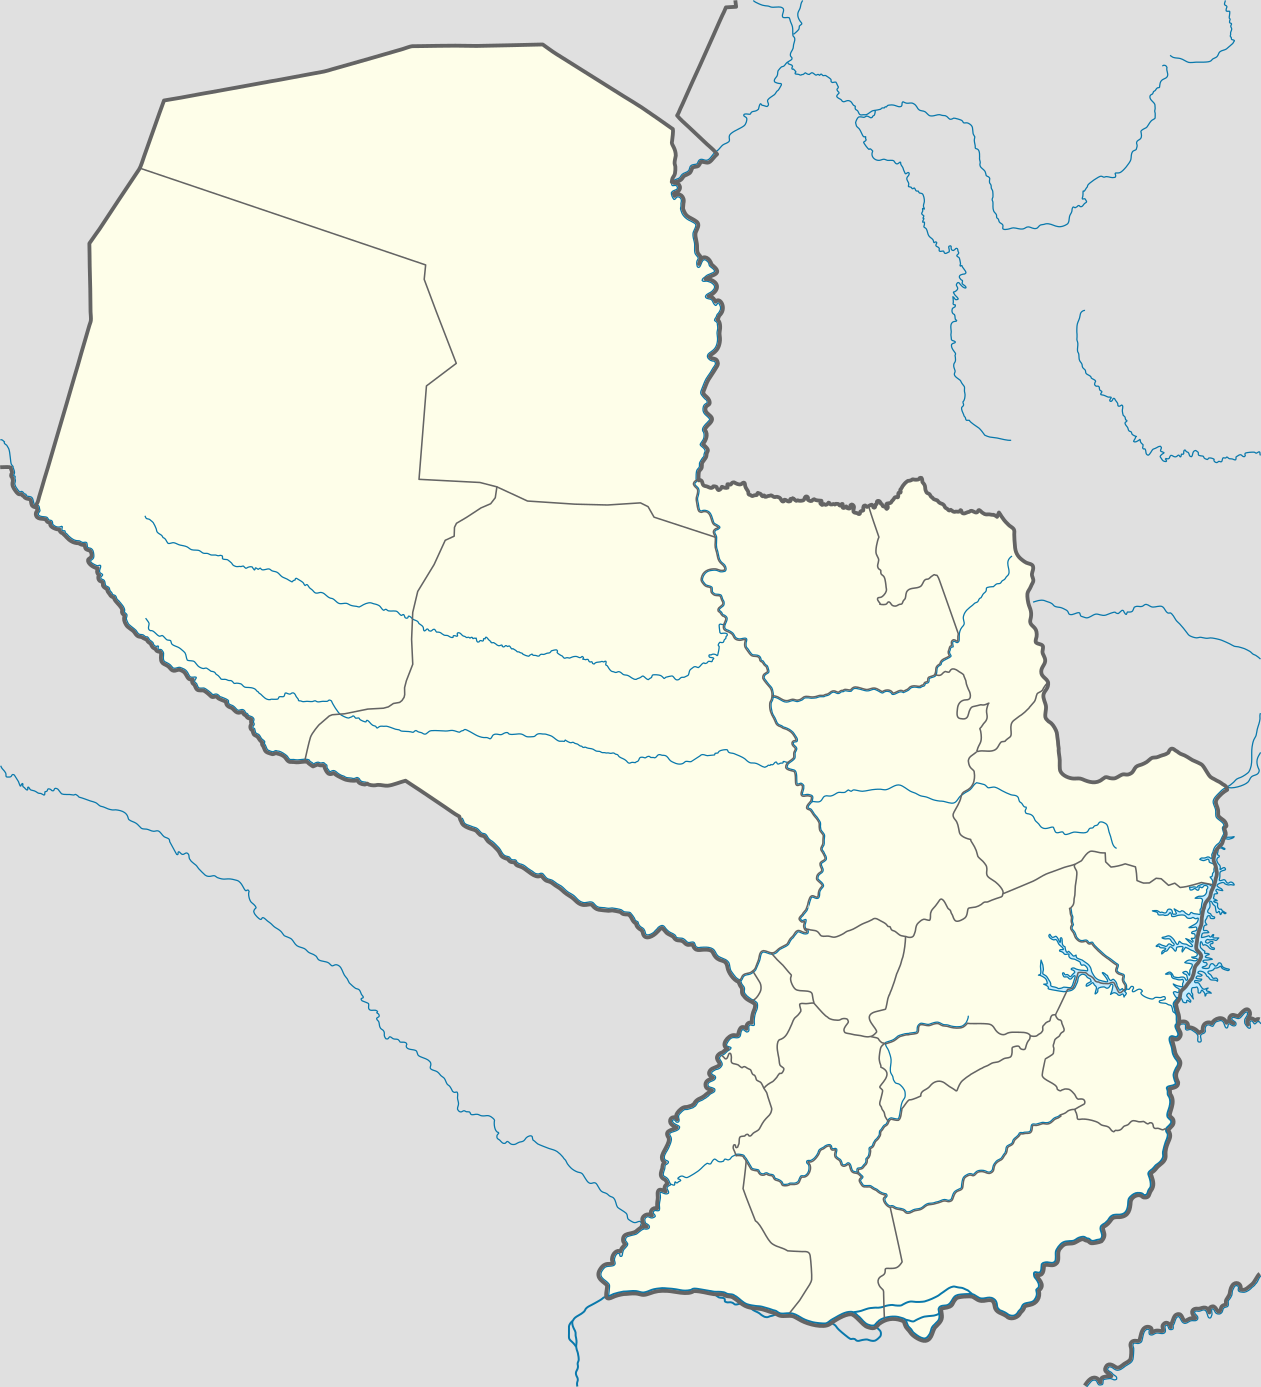
\includegraphics[width=0.33\textwidth]{mapas/paraguai_base.pdf}}{Capiata (Central) apresenta perfil operacional consolidado para
comparacao territorial, com leitura conjunta de infraestrutura, risco
hidroclimatico e capacidade de continuidade de servicos essenciais.

\subsubsection{Por que sim}

\begin{itemize}
\tightlist
\item
  Base institucional de referencia disponivel e rastreavel.
\item
  Estrutura comparativa (A-E/\allowbreak GSS) consistente para decisao relativa.
\item
  Plano de mitigacao acionavel ja definido no dossie.
\end{itemize}

\subsubsection{Por que não}

\begin{itemize}
\tightlist
\item
  Serie oficial distrital granular ainda pode apresentar lacunas
  temporais.
\item
  Sensibilidade do score exige monitoramento continuo de risco e
  conectividade.
\item
  Decisao final depende de validacao de campo e janela temporal recente.
\end{itemize}

\subsubsection{Pre-condicoes Minimas de
Decisao}

\begin{itemize}
\tightlist
\item
  Atualizar indicadores criticos em ciclo trimestral.
\item
  Confirmar trafegabilidade e contingencia hidrica/\allowbreak energetica local.
\item
  Validar checklist de resiliencia domiciliar/\allowbreak logistica antes de decisao
  final.
\end{itemize}

\subsubsection{Recomendação
Técnica}

Uso recomendado como candidato em analise multicriterio, condicionado ao
cumprimento das pre-condicoes acima. Referencia atual de score: GSS 7.1
em 2026-03-05; risco predominante: baixo.}
\begin{table}[ht!]
\small \begin{tabular}{p{3.0cm}p{0.8cm}p{6.0cm}} \toprule
\textbf{Critério} & \textbf{Nota} & \textbf{Justificativa} \\ \midrule
A - Ameaças Estratégicas & 7.0 & - \\
B - Risco Social & 7.3 & - \\
C - Riscos Naturais & 7.1 & - \\
D - Autossuficiência & 6.4 & - \\
E - Institucional & 7.9 & - \\
\midrule \textbf{GSS FINAL} & \textbf{7.1} & \textbf{Seguro (bom potencial com preparacao).} \\ \bottomrule \end{tabular}
\end{table}
\subsubsection{Vulnerabilidades e
Mitigação}\label{vuln-Capiata-vulnerabilidades-e-mitigauxe7uxe3o}

\begin{itemize}
\tightlist
\item
  Exposicao hidrometeorologica controlada (\textless45/\allowbreak 100).
\item
  Conectividade viaria baixa (\textless50/\allowbreak 100).
\item
  Estoque de contingencia para 14 dias (agua/\allowbreak alimentos/\allowbreak combustivel),
  priorizado quando risco hidro=36/\allowbreak 100.
\item
  Duplicar rotas/\allowbreak logistica quando conectividade viaria=37/\allowbreak 100 for
  \textless70; manter rota secundaria mapeada e testada trimestralmente.
\item
  Plano de energia resiliente com autonomia minima de 72h
  (geracao/\allowbreak backup), revisao semestral.
\end{itemize}
\subsubsection{Dossiê de Campo}\label{dossie-Capiata-dossiuxea-de-campo}
\begin{description}[style=nextline,leftmargin=0.5cm,font=\bfseries]
\item[-] N/\allowbreak A
\end{description}
\newpage
\secaoDiagnostico{Fernando de la Mora}{\mapaConteudo{-25.3166}{-57.5333}}{Fernando de la Mora é o coração comercial da Grande Assunção e oferece a
melhor infraestrutura de serviços do país. Sua força absoluta reside na
facilidade de acesso a recursos, saúde e suporte institucional. Contudo,
sua densidade demográfica extrema --- a maior do Paraguai --- a torna
uma das localidades mais vulneráveis do país em cenários de ruptura
social ou desabastecimento urbano. É o local ideal para bases logísticas
e operacionais próximas ao poder central, mas exige um plano de retirada
rigoroso para áreas rurais em caso de crise sistêmica.

\subsubsection{Por que sim}

\begin{itemize}
\tightlist
\item
  Melhor acesso a serviços de saúde, bancos e suprimentos industriais do
  país.
\item
  Conectividade total com a capital e principais eixos rodoviários
  nacionais.
\item
  Segurança institucional forte e infraestrutura urbana moderna.
\item
  Sem restrições da Lei de Fronteira.
\end{itemize}

\subsubsection{Por que não}

\begin{itemize}
\tightlist
\item
  Distrito mais densamente povoado do país (risco social de massa
  elevado).
\item
  Vulnerabilidade total a falhas em redes elétricas e de abastecimento.
\item
  Problemas crônicos de drenagem pluvial (raudales) em tempestades.
\end{itemize}

\subsubsection{Recomendação
Técnica}

Indicado para bases administrativas e logísticas de apoio. Para
residência permanente de refúgio, recomenda-se a estocagem de recursos
para 30 dias e a manutenção de uma rota de fuga secundária para o
departamento de Cordillera ou Paraguarí. O GSS de 6.9 reflete a
excelência dos recursos e serviços em contraste com a extrema
fragilidade demográfica. Referencia atual de score: GSS 6.9 em
2026-03-05.}
\begin{table}[ht!]
\small \begin{tabular}{p{3.0cm}p{0.8cm}p{6.0cm}} \toprule
\textbf{Critério} & \textbf{Nota} & \textbf{Justificativa} \\ \midrule
A - Ameaças Estratégicas & 5.0 & Corredor rodoviário vital para a capital; alvo logístico de visibilidade elevada \\
B - Risco Social & 5.0 & Extrema densidade populacional; risco social e de agitação urbana crítico \\
C - Riscos Naturais & 7.5 & Geologia muito estável e baixo risco de grandes desastres naturais \\
D - Autossuficiência & 8.5 & Melhor infraestrutura comercial e de suprimentos do país; abundância residencial \\
E - Institucional & 8.5 & Forte segurança institucional e serviços de saúde de elite integrados \\
\midrule \textbf{GSS FINAL} & \textbf{6.9} & \textbf{Moderadamente Seguro (Recomendado como base logística e residencial de apoio, não para sobrevivência isolada).} \\ \bottomrule \end{tabular}
\end{table}
\subsubsection{Vulnerabilidades e
Mitigação}\label{vuln-Fernando_de_la_Mora-vulnerabilidades-e-mitigauxe7uxe3o}

\begin{itemize}
\tightlist
\item
  \textbf{Extrema Densidade Demográfica:} Maior risco social do país em
  cenários de fome ou falta de energia (Mitigação: não recomendada para
  refúgio primário; manter apenas como base logística de curto prazo).
\item
  \textbf{Dependência de Redes:} Vulnerabilidade total ao colapso de
  água e luz (Mitigação: instalação de sistemas de energia solar e
  grandes reservatórios de água).
\item
  \textbf{Gargalo Logístico:} Risco de bloqueios totais nas safras da
  capital (Mitigação: mapear rotas de fuga por ruas residenciais
  secundárias).
\end{itemize}
\subsubsection{Dossiê de Campo}\label{dossie-Fernando_de_la_Mora-dossiuxea-de-campo}
\begin{description}[style=nextline,leftmargin=0.5cm,font=\bfseries]
\item[Coordenadas]  25°19'S 57°32'W.
\item[Topografia]  Relevo predominantemente plano, totalmente urbanizado e integrado à mancha urbana de Assunção. Altitude \textasciitilde 140m. Área de \textasciitilde 20 km². Geologicamente muito estável, risco sísmico desprezível.
\item[Alvos Estratégicos]  Corredor Logístico da Ruta PY02 (Eixo vital de entrada/\allowbreak saída da capital); Importantes centros de distribuição e logística comercial (Zona Norte e Sul); Proximidade crítica com sedes administrativas em Assunção. Ausência de bases militares diretas, mas é um ponto de estrangulamento rodoviário tático.
\item[Fallout]  Ventos predominantes do Norte (NE) e Leste. Risco elevado de fallout indireto e contaminação em caso de incidentes severos na capital.
\item[População]  110.255 habitantes (Censo 2022 Final). Uma das cidades mais povoadas e economicamente ativas da região metropolitana.
\item[Densidade]  \textasciitilde 5.512,7 hab/\allowbreak km² (O distrito mais densamente povoado do Paraguai). Indica vulnerabilidade social extrema e risco de desabastecimento crítico em cenários de ruptura sistêmica urbana.
\item[Vias de Acesso]  Cortada pelas principais artérias do país: Ruta PY02 (Mcal. Estigarribia) e Acesso Sul. Conectividade asfáltica total, mas com gargalos de tráfego permanentes. Localização crítica em planos de evacuação.
\item[Serviços]  Infraestrutura de serviços de elite. Sede do Hospital Materno Infantil e proximidade com os melhores hospitais privados do país. Rede bancária e comercial saturada e completa.
\item[Custo de Vida]  Médio-alto; mercado imobiliário extremamente valorizado, sem disponibilidade de terras rurais.
\item[Preço da Terra]  US\$ 150-350/\allowbreak m² (Urbano/\allowbreak Comercial).
\item[Hidrologia]  Risco de Enxurradas Urbanas (Raudales). Problemas crônicos de drenagem pluvial em avenidas principais durante tempestades severas. Baixo risco de inundações fluviais diretas.
\item[Clima]  Subtropical Úmido com forte efeito de ilha de calor urbana. Temperaturas de verão frequentemente superam os 40°C.
\item[Energia]  Rede nacional (Itaipu). Total dependência da integridade da rede metropolitana.
\item[Água]  Sistema ESSAP\footnote{Empresa de Servicios Sanitarios del Paraguay (Empresa de Serviços Sanitários do Paraguai), responsável pelo saneamento e água urbana.} e poços artesianos profundos em condomínios e indústrias.
\item[Qualidade do Solo]  Solo urbano totalmente impermeabilizado; aptidão agrícola nula no distrito.
\item[Resources Locais]  Gigantesco polo comercial e de suprimentos. Contudo, a extrema população gera dependência absoluta de logística externa para alimentação. Resiliência individual depende de estocagem prévia.
\item[Segurança]  Índices de criminalidade urbana típicos de alta densidade metropolitana (assaltos/\allowbreak furtos). Em crises, é uma das zonas de maior risco para distúrbios civis e saques devido à concentração de depósitos e comércio.
\item[Leis Local]  Município consolidado e altamente regulamentado. \\ \textbf{Livre de Restrição} de Fronteira. \\ \textit{Aquisição de terra rural proibida para estrangeiros limítrofes.}
\end{description}
\newpage
\secaoDiagnostico{Guarambare}{\mapaConteudo{-25.4833}{-57.4666}}{Guarambaré é o motor açucareiro do departamento Central. Oferece uma
infraestrutura de serviços sólida e uma capacidade de produção
energética (biocombustíveis) e alimentar regional excepcional. Sua força
absoluta reside na coesão social e na riqueza de seus recursos
agroindustriais. A principal cautela é a densidade demográfica elevada e
a vulnerabilidade como rota de fuga de Assunção, o que exige do ocupante
um posicionamento rural periférico para garantir privacidade e segurança
em cenários de instabilidade metropolitana.

\subsubsection{Por que sim}

\begin{itemize}
\tightlist
\item
  Abundância de recursos energéticos locais (Etanol/\allowbreak Biomassa).
\item
  Solo de alta produtividade e abundância de águas puros via poços.
\item
  Coesão social superior à média metropolitana.
\item
  Sem restrições da Lei de Fronteira.
\end{itemize}

\subsubsection{Por que não}

\begin{itemize}
\tightlist
\item
  Alvo estratégico industrial nacional (Produção de açúcar/\allowbreak combustível).
\item
  Densidade populacional urbana elevada.
\item
  Vulnerável como destino de fluxos migratórios em crises na capital.
\end{itemize}

\subsubsection{Recomendação
Técnica}

Altamente indicado como base logística ou residencial para quem busca
proximidade com a capital com suporte industrial. Requer autonomia
tática e escolha de áreas rurais afastadas do núcleo urbano industrial.
O GSS de 6.4 reflete a solidez dos recursos equilibrada pela
vulnerabilidade demográfica. Referencia atual de score: GSS 6.4 em
2026-03-05.}
\begin{table}[ht!]
\small \begin{tabular}{p{3.0cm}p{0.8cm}p{6.0cm}} \toprule
\textbf{Critério} & \textbf{Nota} & \textbf{Justificativa} \\ \midrule
A - Ameaças Estratégicas & 5.5 & Hub industrial açucareiro e nó logístico secundário; visibilidade estratégica moderada \\
B - Risco Social & 5.5 & População significativa e densidade urbana elevada; risco social em crises metropolitana \\
C - Riscos Naturais & 7.0 & Geologia muito estável e baixo risco de grandes desastres naturais \\
D - Autossuficiência & 7.5 & Excelentes recursos: polo açucareiro, abundância hídrica e solo fértil \\
E - Institucional & 6.5 & Estabilidade institucional e forte coesão social comunitária tradicional \\
\midrule \textbf{GSS FINAL} & \textbf{6.4} & \textbf{Moderadamente Seguro (Ideal como base agroindustrial e de serviços próxima à capital).} \\ \bottomrule \end{tabular}
\end{table}
\subsubsection{Vulnerabilidades e
Mitigação}\label{vuln-Guarambare-vulnerabilidades-e-mitigauxe7uxe3o}

\begin{itemize}
\tightlist
\item
  \textbf{Pressão de Massa:} Por estar na PY01, é destino imediato de
  fluxos migratórios da capital (Mitigação: residência rural afastada
  5-10 km do centro, com autonomia total).
\item
  \textbf{Alvo Tático Industrial:} A usina açucareira é um ponto crítico
  nacional (Mitigação: residência com recuo do perímetro industrial).
\item
  \textbf{Dependência de Redes Metropolitanas:} Vulnerabilidade a falhas
  sistêmicas de energia (Mitigação: aproveitar a biomassa local e
  instalar sistemas solares fotovoltaicos).
\end{itemize}
\subsubsection{Dossiê de Campo}\label{dossie-Guarambare-dossiuxea-de-campo}
\begin{description}[style=nextline,leftmargin=0.5cm,font=\bfseries]
\item[Coordenadas]  25°29'S 57°28'W.
\item[Topografia]  Relevo predominantemente plano a suavemente ondulado. Localizado no sul do departamento Central. Altitude \textasciitilde 110m. Área de \textasciitilde 30 km². Geologicamente muito estável, risco sísmico desprezível.
\item[Alvos Estratégicos]  Ingenio Azucarero Guarambaré (Infraestrutura crítica nacional para produção de açúcar e álcool); Ponto de conexão entre a Ruta PY01 e a Ruta Villeta-Alberdi; Subestação ANDE\footnote{Administración Nacional de Electricidade (Administração Nacional de Eletricidade), companhia estatal de energia.}. Alta importância tática industrial regional.
\item[Fallout]  Ventos predominantes do Norte (NE) e Leste. Baixo risco de fallout direto.
\item[População]  37.245 habitantes (Censo 2022 Final). População urbana consolidada com forte vínculo laboral com a agroindústria.
\item[Densidade]  \textasciitilde 1.241,5 hab/\allowbreak km² (Densidade elevada, indicando vulnerabilidade social e pressão sobre serviços em crises de massa metropolitana).
\item[Vias de Acesso]  Localização estratégica sobre o eixo do Acceso Sur (PY01). Conectividade asfáltica de alta qualidade para Assunção (\textasciitilde 30 km) e para o polo portuário de Villeta. Risco de tornar-se zona de bloqueio e destino imediato de refugiados da capital em crises.
\item[Serviços]  Hospital Distrital elevado à categoria de Hospital Básico em 2025. Infraestrutura urbana organizada, com suporte comercial e financeiro estável.
\item[Custo de Vida]  Baixo; economia impulsionada pelo emprego formal na indústria açucareira e produção de cana.
\item[Preço da Terra]  US\$ 20-50/\allowbreak m² (Urbano); US\$ 15.000-30.000/\allowbreak ha (Rurais/\allowbreak Industriais).
\item[Hidrologia]  Diversos arroios locais. Baixo risco de inundações sistêmicas catastróficas devido ao relevo favorável à drenagem natural. Vulnerabilidade localizada em drenagem pluvial urbana.
\item[Clima]  Subtropical Úmido. Verões intensos (>38°C frequentes).
\item[Energia]  Rede nacional (Itaipu); nodo central de distribuição departamental com alta carga industrial.
\item[Água]  Abundante via poços artesianos profundos e sistemas de junta de saneamento comunitários eficientes.
\item[Qualidade do Solo]  Solo franco-arenoso a argiloso; fértil e profundo, ideal para cana-de-açúcar, mandioca e horticultura familiar.
\item[Resources Locais]  Capital Nacional do Açúcar. Grande excedente de cana-de-açúcar, álcool combustível e biomassa. Elevadíssimo potencial para autossuficiência energética e alimentar básica regional.
\item[Segurança]  Cidade com forte identidade tradicional e cultural. Criminalidade urbana comum presente (furtos), mas monitorada. Coesão social baseada na atividade industrial centenária e festividades tradicionais (Virgen del Rosario). Segurança institucional estável.
\item[Leis Local]  Município consolidado e integrado ao desenvolvimento regional. \\ \textbf{Livre de Restrição} de Fronteira. \\ \textit{Aquisição de terra rural proibida para estrangeiros limítrofes.}
\end{description}
\newpage
\secaoDiagnostico{Ita}{\mapaConteudo{-25.5000}{-57.3500}}{Itá é um dos pilares produtivos e culturais do departamento Central.
Oferece uma infraestrutura de serviços sólida, abundância de recursos
naturais (água e solo para olaria) e uma coesão social baseada na
tradição artesanal que é superior à média metropolitana. Sua força
reside na capacidade de produção de materiais básicos e alimentos de
cinturão verde. A principal cautela reside na densidade demográfica em
ascensão e na exposição direta à Ruta PY01, o que exige um
posicionamento em zonas rurais periféricas para maximizar o isolamento e
a segurança tática.

\subsubsection{Por que sim}

\begin{itemize}
\tightlist
\item
  Abundância de recursos hídricos e solos aptos para policultivos.
\item
  Coesão social e tradição cultural forte (Cidade da Cerâmica).
\item
  Conectividade rápida com Assunção e polos portuários do Sul.
\item
  Sem restrições da Lei de Fronteira.
\end{itemize}

\subsubsection{Por que não}

\begin{itemize}
\tightlist
\item
  Densidade populacional elevada para os padrões de isolamento total.
\item
  Vulnerável como destino imediato de fluxos migratórios em crises na
  capital.
\item
  Infraestrutura de saúde local pode sofrer pressão excessiva em
  cenários de massa.
\end{itemize}

\subsubsection{Recomendação
Técnica}

Altamente indicado para estabelecimentos de autossuficiência de médio
porte que busquem proximidade com a capital. Requer autonomia energética
e hídrica individual e escolha de áreas rurais protegidas do fluxo da
rodovia. O GSS de 6.0 reflete o equilíbrio entre a riqueza de recursos e
a vulnerabilidade demográfica metropolitana. Referencia atual de score:
GSS 6.0 em 2026-03-05.}
\begin{table}[ht!]
\small \begin{tabular}{p{3.0cm}p{0.8cm}p{6.0cm}} \toprule
\textbf{Critério} & \textbf{Nota} & \textbf{Justificativa} \\ \midrule
A - Ameaças Estratégicas & 5.5 & Posicionamento estratégico no eixo PY01; hub artesanal e de suprimentos tático \\
B - Risco Social & 5.5 & População significativa e densidade urbana em crescimento metropolitano \\
C - Riscos Naturais & 7.0 & Geologia muito estável e baixo risco de desastres naturais graves \\
D - Autossuficiência & 7.0 & Bons recursos: polo de cerâmica, hortifrúti e água abundante por poços \\
E - Institucional & 6.0 & Estabilidade institucional e forte coesão social comunitária tradicional \\
\midrule \textbf{GSS FINAL} & \textbf{6.0} & \textbf{Moderadamente Seguro (Ideal para quem busca refúgio rural produtivo próximo à infraestrutura da capital).} \\ \bottomrule \end{tabular}
\end{table}
\subsubsection{Vulnerabilidades e
Mitigação}\label{vuln-Ita-vulnerabilidades-e-mitigauxe7uxe3o}

\begin{itemize}
\tightlist
\item
  \textbf{Pressão Migratória Metropolitana:} Destino óbvio para fluxos
  de Assunção em crises (Mitigação: residência rural afastada 5-10 km do
  centro denso e da rodovia PY01).
\item
  \textbf{Dependência de Redes Públicas:} Vulnerabilidade ao colapso
  sistêmico de energia (Mitigação: instalação de sistemas solares
  fotovoltaicos e armazenamento de água).
\item
  \textbf{Escala Demográfica:} A população de \textasciitilde82k exige
  planejamento de segurança patrimonial rigoroso em cenários de fome
  urbana.
\end{itemize}
\subsubsection{Dossiê de Campo}\label{dossie-Ita-dossiuxea-de-campo}
\begin{description}[style=nextline,leftmargin=0.5cm,font=\bfseries]
\item[Coordenadas]  25°30'S 57°21'W.
\item[Topografia]  Relevo predominantemente plano a suavemente ondulado. Localizado na zona sul do departamento Central. Altitude \textasciitilde 110m. Área de \textasciitilde 182 km². Geologicamente muito estável, risco sísmico desprezível.
\item[Alvos Estratégicos]  Polo de produção de cerâmica e artesanato regional (Capital da Cerâmica); Áreas de horticultura intensiva do cinturão verde metropolitano; Ponto de passagem e fiscalização na Ruta PY01. Ausência de alvos militares diretos, mas estratégico para o suprimento de materiais de construção e alimentos básicos.
\item[Fallout]  Ventos predominantes do Norte (NE) e Leste. Baixo risco de fallout direto.
\item[População]  82.032 habitantes (Censo 2022 Final). População em ritmo de crescimento equilibrado, com forte componente rural preservado.
\item[Densidade]  \textasciitilde 450,7 hab/\allowbreak km² (Densidade elevada, mas inferior à média do núcleo metropolitano de Central, oferecendo melhor isolamento em suas companhias rurais).
\item[Vias de Acesso]  Localização privilegiada sobre o eixo da Ruta PY01 (Acceso Sur). Conectividade asfáltica de elite para Assunção (\textasciitilde 35 km) e para o Sul do país. Risco elevado de tornar-se zona de bloqueio e ponto de convergência de refugiados da capital em crises.
\item[Serviços]  Hospital Distrital de Itá e rede de Unidades de Saúde da Família (USF). Infraestrutura urbana consolidada com comércio diversificado e serviços bancários.
\item[Custo de Vida]  Baixo; economia impulsionada pela agricultura familiar, cerâmica e serviços de trânsito rodoviário.
\item[Preço da Terra]  US\$ 20-50/\allowbreak m² (Urbano); US\$ 15.000-30.000/\allowbreak ha (Rurais/\allowbreak Agrícolas).
\item[Hidrologia]  Baixo risco de inundações sistêmicas catastróficas. Presença da Lagoa de Itá no centro urbano. Vulnerabilidade em drenagem pluvial em bairros baixos durante chuvas intensas (média 1.600 mm/\allowbreak ano).
\item[Clima]  Subtropical Úmido. Verões intensos e invernos amenos.
\item[Energia]  Rede nacional (Itaipu). Total dependência da integridade da rede metropolitana de alta tensão.
\item[Água]  Abundante via poços artesianos profundos e sistemas de junta de saneamento comunitários.
\item[Qualidade do Solo]  Solo argiloso e arenoso (avermelhado); excelente para olaria/\allowbreak cerâmica e muito apto para hortifrúti, mandioca e pastagens.
\item[Resources Locais]  Grande produção de hortaliças, frutas cítricas, mandioca e cerâmica. Elevado potencial para autossuficiência alimentar básica em nível regional e comunitário.
\item[Segurança]  Cidade com forte identidade tradicional e artesanal. Criminalidade urbana comum presente (furtos), típica de periferia metropolitana. Coesão social baseada na cultura da cerâmica e tradições religiosas (San Blas). Segurança institucional estável.
\item[Leis Local]  Município histórico e consolidado. \\ \textbf{Livre de Restrição} de Fronteira. \\ \textit{Aquisição de terra rural proibida para estrangeiros limítrofes.}
\end{description}
\newpage
\secaoDiagnostico{Itaugua}{\mapaConteudo{-25.3833}{-57.3333}}{Itauguá é a fortaleza de saúde e cultura do departamento Central.
Oferece a melhor infraestrutura hospitalar do Paraguai, garantindo um
suporte institucional de elite em qualquer cenário. Sua força reside na
excepcional qualidade de seus recursos (humanos, hídricos e industriais)
e na solidez de sua base cultural baseada no artesanato Ñandutí. É o
local ideal para quem busca proximidade com a capital, mantendo acesso
imediato a serviços vitais, ciente da visibilidade tática do seu polo de
saúde.

\subsubsection{Por que sim}

\begin{itemize}
\tightlist
\item
  Melhor segurança hídrica e hospitalar da região metropolitana.
\item
  Solo de alta produtividade e ambiente social seguro e culturalmente
  coeso.
\item
  Conectividade rápida com Assunção e polos produtivos do Leste.
\item
  Sem restrições da Lei de Fronteira.
\end{itemize}

\subsubsection{Por que não}

\begin{itemize}
\tightlist
\item
  Alvo estratégico hospitalar e logístico em cenários de crise nacional.
\item
  Densidade populacional urbana elevada para um refúgio isolado.
\item
  Dependência tática da Ruta PY02 para mobilidade rápida.
\end{itemize}

\subsubsection{Recomendação
Técnica}

Altamente indicado como base de apoio médico e logístico para o projeto.
Requer posicionamento em zonas rurais distais (10-15 km do centro) para
maximizar a privacidade. O GSS de 7.4 reflete a excepcional força dos
recursos e da segurança institucional da localidade. Referencia atual de
score: GSS 7.4 em 2026-03-05.}
\begin{table}[ht!]
\small \begin{tabular}{p{3.0cm}p{0.8cm}p{6.0cm}} \toprule
\textbf{Critério} & \textbf{Nota} & \textbf{Justificativa} \\ \midrule
A - Ameaças Estratégicas & 6.0 & Hub de saúde e logístico vital; alvo estratégico tático de alta visibilidade e proteção \\
B - Risco Social & 6.0 & População regional elevada e densidade urbana manejada para o padrão Central \\
C - Riscos Naturais & 7.0 & Geologia muito estável e baixo risco de grandes desastres naturais \\
D - Autossuficiência & 8.5 & Recursos agroindustriais e hídricos excepcionais; solo de elite e polo têxtil \\
E - Institucional & 8.5 & Fortíssima segurança institucional e melhor suporte hospitalar do país \\
\midrule \textbf{GSS FINAL} & \textbf{7.4} & \textbf{Seguro (Localidade altamente recomendada como base de suporte médico e logístico para o projeto).} \\ \bottomrule \end{tabular}
\end{table}
\subsubsection{Vulnerabilidades e
Mitigação}\label{vuln-Itaugua-vulnerabilidades-e-mitigauxe7uxe3o}

\begin{itemize}
\tightlist
\item
  \textbf{Pressão Administrativa e de Saúde:} O Hospital Nacional é um
  alvo tático em crises sanitárias ou humanitárias (Mitigação:
  residência rural afastada 10-15 km do complexo hospitalar).
\item
  \textbf{Exposição Rodoviária:} Localização direta na PY02 atrai fluxos
  de trânsito intenso em crises (Mitigação: residência com acesso por
  múltiplas rotas rurais secundárias).
\item
  \textbf{Dependência de Redes Públicas:} Vulnerabilidade ao colapso
  sistêmico de energia (Mitigação: instalação de sistemas solares
  fotovoltaicos potentes).
\end{itemize}
\subsubsection{Dossiê de Campo}\label{dossie-Itaugua-dossiuxea-de-campo}
\begin{description}[style=nextline,leftmargin=0.5cm,font=\bfseries]
\item[Coordenadas]  25°23'S 57°20'W.
\item[Topografia]  Relevo predominantemente plano com suaves ondulações. Localizado estrategicamente no centro-leste do departamento Central. Altitude \textasciitilde 170m. Área de \textasciitilde 122 km². Geologicamente muito estável, risco sísmico desprezível.
\item[Alvos Estratégicos]  Hospital Nacional de Itauguá (O maior centro de referência médica do país, infraestrutura crítica de saúde); Polo industrial têxtil e de confecções (Ñandutí); Importante nó logístico na Ruta PY02 duplicada. Alta visibilidade institucional e de serviços.
\item[Fallout]  Ventos predominantes do Norte (NE) e Leste. Risco de fallout indireto moderado em caso de ataques severos à capital Assunção (\textasciitilde 35 km).
\item[População]  111.203 habitantes (Censo 2022 Final). Distrito com forte componente demográfico jovem e em plena expansão residencial/\allowbreak industrial.
\item[Densidade]  \textasciitilde 911,5 hab/\allowbreak km² (Densidade urbana elevada, indicando vulnerabilidade social e pressão sobre serviços em crises de massa metropolitana).
\item[Vias de Acesso]  Localização privilegiada sobre o eixo da Ruta PY02 duplicada. Conectividade asfáltica de elite para Assunção e para o Leste (CDE). Risco elevado de tornar-se zona de controle e ponto de convergência de refugiados em crises nacionais.
\item[Serviços]  Melhor infraestrutura de saúde pública do interior (Hospital Nacional). Rede bancária, comercial e educacional (Polo Universitário) robusta e consolidada.
\item[Custo de Vida]  Médio; economia impulsionada pela indústria, artesanato e comércio de trânsito.
\item[Preço da Terra]  US\$ 40-90/\allowbreak m² (Urbano); US\$ 30.000-60.000/\allowbreak ha (Zonas industriais mecanizadas).
\item[Hidrologia]  Diversos arroios cruzam o distrito. Baixo risco de inundações sistêmicas catastróficas devido ao relevo favorável. Vulnerabilidade localizada em drenagem pluvial urbana durante tempestades severas (média 1.600 mm/\allowbreak ano).
\item[Clima]  Subtropical Úmido. Verões intensos e úmidos.
\item[Energia]  Rede nacional (Itaipu); nodo importante de distribuição regional com alta carga industrial.
\item[Água]  Abundante via poços artesianos profundos e sistemas de junta de saneamento comunitários eficientes.
\item[Qualidade do Solo]  Solo franco-argiloso (avermelhado); muito fértil e profundo, ideal para fruticultura, mandioca e pastagens cultivadas.
\item[Resources Locais]  Grande polo produtor de artesanato têxtil (Ñandutí), hortifrúti e indústria de confecções. Elevado potencial para autossuficiência alimentar básica regional, embora dependente de logística interna.
\item[Segurança]  Cidade próspera com segurança social estável para o padrão metropolitano. Criminalidade urbana comum presente (furtos), mas sob vigilância tática devido à importância do Hospital Nacional e polos industriais. Coesão social baseada na identidade cultural do Ñandutí.
\item[Leis Local]  Município consolidado e polo de referência em saúde. \\ \textbf{Livre de Restrição} de Fronteira. \\ \textit{Aquisição de terra rural proibida para estrangeiros limítrofes.}
\end{description}
\newpage
\secaoDiagnostico{J Augusto Saldivar}{\mapaConteudo{-25.4500}{-57.4166}}{J. Augusto Saldívar é o ``celeiro'' hortícola da região metropolitana.
Oferece uma infraestrutura de serviços básica, mas compensada pela
excepcional abundância de recursos alimentares frescos e solos férteis.
Sua força reside na capacidade de produção alimentar de cinturão verde e
na segurança hídrica via poços profundos. A principal cautela é sua
localização estratégica na Ruta PY01, o que exige um posicionamento em
zonas rurais afastadas do eixo asfáltico para maximizar a privacidade e
a segurança tática em cenários de instabilidade metropolitana.

\subsubsection{Por que sim}

\begin{itemize}
\tightlist
\item
  Abundância de recursos alimentares (frutas e verduras) e hídricos.
\item
  Ambiente social mais tranquilo que o núcleo denso da Grande Assunção.
\item
  Conectividade rápida com a capital e com o interior produtivo do Sul.
\item
  Sem restrições da Lei de Fronteira.
\end{itemize}

\subsubsection{Por que não}

\begin{itemize}
\tightlist
\item
  Densidade populacional elevada para os padrões de isolamento total.
\item
  Vulnerável como destino de fluxos migratórios em crises na capital.
\item
  Dependência de serviços hospitalares especializados em cidades
  vizinhas.
\end{itemize}

\subsubsection{Recomendação
Técnica}

Altamente indicado para estabelecimentos de autossuficiência familiar
que priorizem a segurança alimentar e busquem proximidade com a
infraestrutura da capital. Requer autonomia energética individual e
escolha de áreas rurais protegidas. O GSS de 6.8 reflete a solidez dos
recursos alimentares equilibrada pela vulnerabilidade demográfica
metropolitana. Referencia atual de score: GSS 6.8 em 2026-03-05.}
\begin{table}[ht!]
\small \begin{tabular}{p{3.0cm}p{0.8cm}p{6.0cm}} \toprule
\textbf{Critério} & \textbf{Nota} & \textbf{Justificativa} \\ \midrule
A - Ameaças Estratégicas & 5.5 & Posicionamento estratégico no eixo PY01; hub de suprimentos tático alimentar \\
B - Risco Social & 6.0 & População moderada e densidade manejada para o padrão Central; baixo risco social \\
C - Riscos Naturais & 7.0 & Geologia muito estável e baixo risco de grandes desastres naturais \\
D - Autossuficiência & 8.5 & Recursos alimentares excepcionais: cinturão verde de hortifrúti e água por poços \\
E - Institucional & 6.5 & Estabilidade institucional e segurança social comunitária estável \\
\midrule \textbf{GSS FINAL} & \textbf{6.8} & \textbf{Moderadamente Seguro (Ideal para quem busca refúgio rural produtivo próximo à capital com foco em segurança alimentar).} \\ \bottomrule \end{tabular}
\end{table}
\subsubsection{Vulnerabilidades e
Mitigação}\label{vuln-J_Augusto_Saldivar-vulnerabilidades-e-mitigauxe7uxe3o}

\begin{itemize}
\tightlist
\item
  \textbf{Pressão Migratória Metropolitana:} Por estar no eixo PY01, é
  destino provável de fluxos de Assunção (Mitigação: residência rural
  afastada 3-5 km do centro denso e da rodovia).
\item
  \textbf{Dependência de Redes Públicas:} Vulnerabilidade ao colapso
  sistêmico de energia para irrigação (Mitigação: instalação de sistemas
  solares fotovoltaicos e reservatórios de água).
\item
  \textbf{Escala Comercial:} Dependência de centros vizinhos para
  serviços hospitalares avançados (Mitigação: manutenção de estoque
  médico básico e kit trauma local).
\end{itemize}
\subsubsection{Dossiê de Campo}\label{dossie-J_Augusto_Saldivar-dossiuxea-de-campo}
\begin{description}[style=nextline,leftmargin=0.5cm,font=\bfseries]
\item[Coordenadas]  25°27'S 57°25'W.
\item[Topografia]  Relevo predominantemente plano, localizado em zona de transição entre o núcleo metropolitano e as áreas rurais do Sul. Altitude \textasciitilde 120m. Área de \textasciitilde 32 km². Geologicamente muito estável, risco sísmico desprezível.
\item[Alvos Estratégicos]  Eixo logístico vital da Ruta PY01 (Acceso Sur); Polo de fornecimento hortícola massivo para a Grande Assunção; Subestação da ANDE\footnote{Administración Nacional de Electricidade (Administração Nacional de Eletricidade), companhia estatal de energia.}. Ausência de alvos militares de grande porte, mas estratégico para o controle de suprimentos alimentares da capital.
\item[Fallout]  Ventos predominantes do Norte (NE) e Leste. Baixo risco de fallout direto.
\item[População]  56.525 habitantes (Censo 2022 Final). Crescimento populacional moderado comparado a distritos vizinhos, mantendo perfil urbano-rural.
\item[Densidade]  \textasciitilde 1.766,4 hab/\allowbreak km² (Densidade elevada, indicando vulnerabilidade social e pressão sobre serviços em crises de massa metropolitana).
\item[Vias de Acesso]  Localização privilegiada sobre a Ruta PY01. Conectividade asfáltica de elite para Assunção (\textasciitilde 25 km) e para o Sul do país. Risco elevado de tornar-se zona de bloqueio e ponto de concentração de refugiados da capital em crises.
\item[Serviços]  Infraestrutura urbana básica a média. Unidade de Saúde da Família (USF) local. Dependência de Capiatá ou Itá para atendimentos médicos de alta complexidade.
\item[Custo de Vida]  Baixo para o padrão metropolitano; economia impulsionada pela pequena agricultura e comércio de beira de estrada.
\item[Preço da Terra]  US\$ 15-40/\allowbreak m² (Urbano); US\$ 30.000-50.000/\allowbreak ha (Rurais/\allowbreak Agrícolas).
\item[Hidrologia]  Baixo risco de inundações sistêmicas catastróficas. Vulnerabilidade localizada em drenagem pluvial urbana durante tempestades severas (média 1.600 mm/\allowbreak ano).
\item[Clima]  Subtropical Úmido. Verões intensos com alta umidade.
\item[Energia]  Rede nacional (Itaipu). Dependência total da integridade da rede metropolitana de Central.
\item[Água]  Abundante via poços artesianos profundos e sistemas de junta de saneamento comunitários.
\item[Qualidade do Solo]  Solo franco-arenoso a argiloso; muito fértil e apto para horticultura intensiva, mandioca e frutas.
\item[Resources Locais]  Cinturão Verde de Assunção. Grande produção de hortaliças, legumes e frutas que abastecem o Mercado de Abasto. Elevado potencial para autossuficiência alimentar básica regional e familiar.
\item[Segurança]  Zona residencial e agrícola pacífica para o padrão de Central. Criminalidade urbana comum presente, mas monitorada. Coesão social baseada na cultura da pequena agricultura e comércio familiar. Segurança institucional estável.
\item[Leis Local]  Município consolidado. \\ \textbf{Livre de Restrição} de Fronteira. \\ \textit{Aquisição de terra rural proibida para estrangeiros limítrofes.}
\end{description}
\newpage
\secaoDiagnostico{Lambare}{\mapaConteudo{-25.3333}{-57.6166}}{Lambaré é a principal zona residencial de elite da Grande Assunção.
Oferece infraestrutura de serviços e segurança institucional de nível
superior, beneficiando-se da continuidade urbana com a capital. Sua
força reside na alta qualidade de vida e no suporte estatal robusto.
Contudo, sua extrema densidade populacional e a dependência absoluta de
redes externas a tornam vulnerável em cenários de colapso sistêmico
nacional. É o local ideal para quem busca segurança social e proximidade
com o poder central, exigindo investimento em autonomia individual de
recursos.

\subsubsection{Por que sim}

\begin{itemize}
\tightlist
\item
  Melhor infraestrutura residencial e acesso a serviços de elite do
  país.
\item
  Ambiente social seguro em zonas consolidadas com segurança privada.
\item
  Geologia extremamente estável e conectividade total.
\item
  Sem restrições da Lei de Fronteira.
\end{itemize}

\subsubsection{Por que não}

\begin{itemize}
\tightlist
\item
  Densidade populacional elevada (risco social de massa em crises).
\item
  Primeiro destino provável para refugiados de Assunção.
\item
  Vulnerabilidade total a falhas em redes elétricas e de abastecimento
  hídrico.
\end{itemize}

\subsubsection{Recomendação
Técnica}

Altamente indicado como base residencial de alto padrão próxima à
capital. Exige planejamento de autonomia hídrica (poços profundos),
energética (solar) e estocagem robusta para 30-60 dias. O GSS de 7.3
reflete a excepcional solidez institucional equilibrada pela fragilidade
demográfica metropolitana. Referencia atual de score: GSS 7.3 em
2026-03-05.}
\begin{table}[ht!]
\small \begin{tabular}{p{3.0cm}p{0.8cm}p{6.0cm}} \toprule
\textbf{Critério} & \textbf{Nota} & \textbf{Justificativa} \\ \midrule
A - Ameaças Estratégicas & 5.5 & Proximidade crítica com a capital; vulnerável como rota de escape metropolitana \\
B - Risco Social & 5.0 & Densidade urbana elevada e população significativa; risco social em crises de massa \\
C - Riscos Naturais & 7.5 & Geologia muito estável e baixo risco de grandes desastres naturais \\
D - Autossuficiência & 8.5 & Melhor infraestrutura de serviços e suprimentos do país adjacente \\
E - Institucional & 8.5 & Forte segurança institucional e social sustentada pelo perfil residencial de elite \\
\midrule \textbf{GSS FINAL} & \textbf{7.0
7.3} & \textbf{Seguro (Indicado como base residencial de elite próxima à capital, ciente da vulnerabilidade demográfica).} \\ \bottomrule \end{tabular}
\end{table}
\subsubsection{Vulnerabilidades e
Mitigação}\label{vuln-Lambare-vulnerabilidades-e-mitigauxe7uxe3o}

\begin{itemize}
\tightlist
\item
  \textbf{Pressão Demográfica Crítica:} Por ser colada à capital, é
  destino imediato de fluxos migratórios em crises (Mitigação: não
  recomendada para refúgio primário; manter apenas base residencial
  tática com fortificação física).
\item
  \textbf{Dependência de Redes Metropolitanas:} Vulnerabilidade total ao
  colapso de água e luz (Mitigação: instalação de sistemas solares
  potentes e grandes reservatórios de água independentes).
\item
  \textbf{Isolamento em Crises:} Risco de bloqueio total de acessos para
  a capital (Mitigação: posse de embarcação leve para via fluvial no Rio
  Paraná como rota alternativa).
\end{itemize}
\subsubsection{Dossiê de Campo}\label{dossie-Lambare-dossiuxea-de-campo}
\begin{description}[style=nextline,leftmargin=0.5cm,font=\bfseries]
\item[Coordenadas]  25°20'S 57°37'W.
\item[Topografia]  Relevo ondulado com colinas que oferecem vista panorâmica para o Rio Paraná e Assunção. Altitude \textasciitilde 150m. Área de \textasciitilde 27 km². Geologicamente estável, risco sísmico desprezível.
\item[Alvos Estratégicos]  Polo residencial de alto padrão da Grande Assunção; Sede do Yacht y Golf Club Paraguayo (infraestrutura social de elite); Proximidade crítica com o Cerro Lambaré (valor simbólico e tático). Ausência de alvos militares diretos, mas alta visibilidade social por abrigar parte da elite econômica nacional.
\item[Fallout]  Ventos predominantes do Norte (NE) e Leste. Risco de fallout indireto elevado em caso de incidentes severos na capital Assunção (continuidade urbana total).
\item[População]  127.150 habitantes (Censo 2022 Final). Cidade essencialmente residencial e comercial, integrada à região metropolitana.
\item[Densidade]  \textasciitilde 4.709,3 hab/\allowbreak km² (Densidade urbana muito elevada, indicando vulnerabilidade social crítica e pressão sobre serviços em cenários de ruptura sistêmica).
\item[Vias de Acesso]  Excelente conectividade asfáltica. Principais eixos via Av. Cacique Lambaré, Av. Juan Perón e Av. Carretera de López. Risco extremo de saturação rodoviária absoluta em crises de evacuação da capital.
\item[Serviços]  Infraestrutura de serviços de elite. Hospital Distrital de Lambaré e proximidade imediata com os melhores sanatórios privados de Assunção. Rede bancária, escolar e comercial saturada e completa.
\item[Custo de Vida]  Alto; mercado imobiliário extremamente valorizado em zonas residenciais consolidadas.
\item[Preço da Terra]  US\$ 100-250/\allowbreak m² (Urbano/\allowbreak Residencial).
\item[Hidrologia]  Risco de Enxurradas Urbanas (Raudales). Problemas crônicos de drenagem pluvial em avenidas durante tempestades severas. Baixo risco de inundações fluviais diretas na maior parte do território, exceto em áreas muito baixas próximas à orla do rio.
\item[Clima]  Subtropical Úmido. Verões intensos com forte efeito de ilha de calor urbana.
\item[Energia]  Rede nacional (Itaipu). Total dependência da integridade da rede metropolitana.
\item[Água]  Sistema ESSAP\footnote{Empresa de Servicios Sanitarios del Paraguay (Empresa de Serviços Sanitários do Paraguai), responsável pelo saneamento e água urbana.} e poços artesianos profundos em condomínios residenciais.
\item[Qualidade do Solo]  Solo urbano impermeabilizado; aptidão agrícola nula no distrito.
\item[Resources Locais]  Cidade focada em serviços e residência. Resiliência e autossuficiência nulas a nível distrital. Dependência absoluta de logística externa (Mercado de Abasto) para alimentação.
\item[Segurança]  Zona residencial consolidada com forte presença de segurança privada. Criminalidade urbana comum presente (furtos/\allowbreak assaltos), mas com policiamento ostensivo. Estabilidade social alta em bairros residenciais, desafiada por focos de vulnerabilidade periférica.
\item[Leis Local]  Município consolidado e altamente regulamentado. \\ \textbf{Livre de Restrição} de Fronteira. \\ \textit{Aquisição de terra rural proibida para estrangeiros limítrofes.}
\end{description}
\newpage
\secaoDiagnostico{Limpio}{\mapaConteudo{-25.1833}{-57.4833}}{Limpio é o portão norte da Grande Assunção e oferece uma infraestrutura
logística e comercial em plena expansão. Sua força reside na facilidade
de acesso a suprimentos e na sua importância como nó de conexão para o
interior do país. Contudo, sua extrema vulnerabilidade hidrológica
(áreas de pântanos e risco de cheias) e a alta densidade demográfica a
tornam um local de risco elevado em cenários de instabilidade sistêmica
ou eventos climáticos extremos. É o local ideal para bases logísticas
comerciais, exigindo do ocupante uma escolha técnica rigorosa de
terrenos em cotas de segurança contra inundações.

\subsubsection{Por que sim}

\begin{itemize}
\tightlist
\item
  Melhor acesso logístico para o Norte e para a capital.
\item
  Solo apto para horticultura familiar e abundância de águas via poços.
\item
  Infraestrutura comercial diversificada e em crescimento.
\item
  Sem restrições da Lei de Fronteira.
\end{itemize}

\subsubsection{Por que não}

\begin{itemize}
\tightlist
\item
  Distrito com alto risco de inundações fluviais e raudales urbanos.
\item
  Alta densidade demográfica favorece o caos social em crises de
  suprimento.
\item
  Alvo estratégico logístico de visibilidade elevada na PY03.
\end{itemize}

\subsubsection{Recomendação
Técnica}

Indicado como hub logístico ou base de apoio. Para residência
permanente, recomenda-se a zona rural do distrito em cotas de altitude
superiores, mantendo autonomia hídrica e energética. O GSS de 6.5
reflete o poder dos recursos e logística equilibrado pela fragilidade
ambiental e tática. Referencia atual de score: GSS 6.5 em 2026-03-05.}
\begin{table}[ht!]
\small \begin{tabular}{p{3.0cm}p{0.8cm}p{6.0cm}} \toprule
\textbf{Critério} & \textbf{Nota} & \textbf{Justificativa} \\ \midrule
A - Ameaças Estratégicas & 5.0 & Hub logístico vital na PY03; alvo tático como via de saída da capital \\
B - Risco Social & 5.5 & População elevada e densidade crítica; alto risco social em crises metropolitana \\
C - Riscos Naturais & 5.5 & Geologia estável; nota penalizada pelo risco crítico de inundação fluvial e pluvial \\
D - Autossuficiência & 7.5 & Excelentes recursos: hub de logística regional, suprimentos comerciais e água abundante \\
E - Institucional & 6.5 & Estabilidade institucional e segurança regional metropolitana funcional \\
\midrule \textbf{GSS FINAL} & \textbf{6.0
6.5} & \textbf{Moderadamente Seguro (Ideal como base logística de apoio, ciente dos riscos hidrológicos e demográficos).} \\ \bottomrule \end{tabular}
\end{table}
\subsubsection{Vulnerabilidades e
Mitigação}\label{vuln-Limpio-vulnerabilidades-e-mitigauxe7uxe3o}

\begin{itemize}
\tightlist
\item
  \textbf{Vulnerabilidade Hidrológica Extrema:} Risco de inundações
  fluviais e pluviais (Mitigação: construção exclusivamente em cotas
  elevadas \textgreater110m e longe das margens do Rio Salado/\allowbreak Paraguai).
\item
  \textbf{Pressão Migratória de Saída:} Rota principal de escape da
  capital para o Norte (Mitigação: residência rural afastada 5-10 km da
  Ruta PY03, com sistemas de segurança tática).
\item
  \textbf{Dependência de Redes Públicas:} Vulnerabilidade total ao
  colapso de energia e abastecimento alimentar externo (Mitigação:
  instalação de sistemas solares fotovoltaicos e estocagem robusta para
  30 dias).
\end{itemize}
\subsubsection{Dossiê de Campo}\label{dossie-Limpio-dossiuxea-de-campo}
\begin{description}[style=nextline,leftmargin=0.5cm,font=\bfseries]
\item[Coordenadas]  25°11'S 57°29'W.
\item[Topografia]  Relevo de planície com áreas de pântanos e baixadas, margeado pelo Rio Paraguai e Rio Salado. Altitude \textasciitilde 100m. Área de \textasciitilde 106 km². Geologicamente estável, risco sísmico muito baixo.
\item[Alvos Estratégicos]  Portal de Entrada para o Norte (Início da Ruta PY03); Polo logístico industrial e de distribuição; Humedais do Rio Paraguai (ativo ambiental); Proximidade com o Rio Salado. Ausência de alvos militares de grande escala, mas ponto de controle tático logístico na Grande Assunção.
\item[Fallout]  Ventos predominantes do Norte (NE) e Leste. Baixo risco de fallout direto.
\item[População]  139.652 habitantes (Censo 2022 Final). Uma das cidades com maior crescimento demográfico absoluto e expansão de loteamentos populares na região metropolitana.
\item[Densidade]  \textasciitilde 1.317,5 hab/\allowbreak km² (Densidade elevada, indicando alta vulnerabilidade social e pressão sobre serviços básicos em cenários de crises de massa).
\item[Vias de Acesso]  Cortada pela Ruta PY03. Principal artéria de conexão entre a capital e o departamento de San Pedro e o Norte do país. Risco extremo de paralisia total das rotas em caso de fuga massiva de Assunção (\textasciitilde 25 km).
\item[Serviços]  Hospital Distrital de Limpio e rede comercial em rápida expansão. Polo de centros de distribuição (logística de varejo). Infraestrutura de saúde pressionada pelo crescimento populacional.
\item[Custo de Vida]  Baixo; economia baseada no comércio, logística e serviços metropolitanos.
\item[Preço da Terra]  US\$ 30-80/\allowbreak m² (Urbano); US\$ 40.000-60.000/\allowbreak ha (Zonas rurais/\allowbreak loteamentos).
\item[Hidrologia]  Risco Crítico de Inundação. Grandes áreas do distrito são baixadas ou pântanos vulneráveis às cheias do Rio Paraguai e Rio Salado. Problemas recorrentes de drenagem pluvial urbana (raudales) em tempestades severas.
\item[Clima]  Subtropical Úmido. Verões intensos (>38°C frequentes) com alta umidade.
\item[Energia]  Rede nacional (Itaipu). Total dependência da integridade da rede metropolitana.
\item[Água]  Sistema ESSAP\footnote{Empresa de Servicios Sanitarios del Paraguay (Empresa de Serviços Sanitários do Paraguai), responsável pelo saneamento e água urbana.} e poços artesianos profundos. Água superficial altamente vulnerável a contaminação em áreas baixas.
\item[Qualidade do Solo]  Solo arenoso e hidromórfico; fértil para horticultura, mas com limitações de drenagem que dificultam a agricultura mecanizada intensiva.
\item[Resources Locais]  Grande polo de logística e suprimentos comerciais. Produção hortícola remanescente, mas insuficiente para a massa populacional urbana. Baixa capacidade de autossuficiência calórica total no distrito.
\item[Segurança]  Cidade dinâmica com índices de criminalidade urbana típicos de áreas de crescimento rápido e desordenado. Vulnerabilidade a delitos contra o patrimônio e insegurança em áreas periféricas. Segurança institucional presente, mas sob pressão demográfica.
\item[Leis Local]  Município consolidado. \\ \textbf{Livre de Restrição} de Fronteira. \\ \textit{Aquisição de terra rural proibida para estrangeiros limítrofes.}
\end{description}
\newpage
\secaoDiagnostico{Luque}{\mapaConteudo{-25.2666}{-57.4833}}{Luque é o epicentro da conectividade aérea e militar do Paraguai.
Oferece infraestrutura de serviços e segurança estatal de nível
superior, garantindo uma base operacional estável em tempos de
normalidade. Sua força reside na excepcional concentração de recursos
tecnológicos e forças de segurança. Contudo, sua importância estratégica
como a principal porta de entrada do país a torna um alvo tático de
altíssima visibilidade em cenários de conflito. É o local ideal para
quem busca infraestrutura de elite e proximidade com a capital, exigindo
do ocupante planos de contingência tática e autonomia de suprimentos
fora do núcleo denso.

\subsubsection{Por que sim}

\begin{itemize}
\tightlist
\item
  Melhor infraestrutura de transporte e logística aérea do país.
\item
  Presença permanente de forças militares e policiais de elite.
\item
  Abundância de recursos industriais e serviços de alta complexidade.
\item
  Sem restrições da Lei de Fronteira.
\end{itemize}

\subsubsection{Por que não}

\begin{itemize}
\tightlist
\item
  Alvo estratégico prioritário nacional (Aeroporto e Bases Militares).
\item
  Densidade populacional elevada favorece riscos sociais em crises.
\item
  Vulnerabilidade a bloqueios táticos nos eixos de conexão com Assunção.
\end{itemize}

\subsubsection{Recomendação
Técnica}

Altamente indicado como base logística ou administrativa de elite. Para
moradia permanente, recomenda-se a zona rural do distrito ou áreas
próximas aos limites com Areguá/\allowbreak Limpio, mantendo autonomia hídrica e
energética. O GSS de 6.7 reflete o poder da infraestrutura tática
equilibrado pela extrema visibilidade do alvo. Referencia atual de
score: GSS 6.7 em 2026-03-05.}
\begin{table}[ht!]
\small \begin{tabular}{p{3.0cm}p{0.8cm}p{6.0cm}} \toprule
\textbf{Critério} & \textbf{Nota} & \textbf{Justificativa} \\ \midrule
A - Ameaças Estratégicas & 4.0 & Alvo estratégico primário: aeroporto e bases militares; altíssima visibilidade tática \\
B - Risco Social & 5.0 & População massiva e densidade elevada; risco social e de agitação urbana significativo \\
C - Riscos Naturais & 7.0 & Geologia muito estável e riscos naturais climáticos manejáveis \\
D - Autossuficiência & 8.0 & Recursos industriais e hídricos excepcionais; hub tecnológico e de aviação \\
E - Institucional & 8.0 & Forte segurança institucional e presença de forças de segurança de elite permanente \\
\midrule \textbf{GSS FINAL} & \textbf{6.2
6.7} & \textbf{Moderadamente Seguro (Ideal como base logística e operacional de alto padrão, requer preparo para visibilidade estratégica).} \\ \bottomrule \end{tabular}
\end{table}
\subsubsection{Vulnerabilidades e
Mitigação}\label{vuln-Luque-vulnerabilidades-e-mitigauxe7uxe3o}

\begin{itemize}
\tightlist
\item
  \textbf{Alvo Estratégico Primário:} O aeroporto e a base aérea são
  alvos militares obrigatórios em conflitos (Mitigação: residência rural
  afastada 15-20 km dos perímetros militares e aeroportuários).
\item
  \textbf{Concentração Populacional:} Risco de instabilidade social e
  saques em crises agudas de suprimento (Mitigação: estabelecimento de
  base em condomínios com segurança privada robusta e autonomia
  alimentar).
\item
  \textbf{Dependência de Redes:} Vulnerabilidade total ao colapso de
  serviços metropolitanos (Mitigação: instalação de sistemas solares
  potentes e poço artesiano próprio).
\end{itemize}
\subsubsection{Dossiê de Campo}\label{dossie-Luque-dossiuxea-de-campo}
\begin{description}[style=nextline,leftmargin=0.5cm,font=\bfseries]
\item[Coordenadas]  25°16'S 57°29'W.
\item[Topografia]  Relevo predominantemente plano a suavemente ondulado. Localizado no núcleo central do departamento Central. Altitude \textasciitilde 120m. Área de \textasciitilde 203 km². Geologicamente muito estável, risco sísmico desprezível.
\item[Alvos Estratégicos]  Aeroporto Internacional Silvio Pettirossi (A principal porta de entrada e saída do país); Base Aérea de Ñu Guazú (Comando da Força Aérea Paraguaia); Sede da CONMEBOL; Parque Ñu Guazú (Espaço tático para logística de emergência e heliportos). Alta visibilidade militar e estratégica internacional.
\item[Fallout]  Ventos predominantes do Norte (NE) e Leste. Risco elevado de fallout em caso de ataques a centros de comando metropolitano.
\item[População]  259.705 habitantes (Censo 2022 Final). Terceira cidade mais populosa do Paraguai e motor do crescimento metropolitano.
\item[Densidade]  \textasciitilde 1.279,3 hab/\allowbreak km² (Densidade urbana elevada, indicando alta vulnerabilidade social e pressão sobre serviços em crises de massa).
\item[Vias de Acesso]  Eixo de conexão vital com Assunção via Autopista Silvio Pettirossi e Av. Aviadores del Chaco. Conectividade asfáltica de elite, mas com gargalos táticos em pontes e cruzamentos em cenários de evacuação.
\item[Serviços]  Infraestrutura de saúde robusta (Hospital Regional, Hospital de Trauma em proximidade, Clínicas privadas de alta complexidade). Polo comercial, financeiro e industrial consolidado.
\item[Custo de Vida]  Médio; economia impulsionada pela aviação, indústria e serviços especializados.
\item[Preço da Terra]  US\$ 50-150/\allowbreak m² (Urbano); US\$ 40.000-80.000/\allowbreak ha (Zonas rurais/\allowbreak industriais).
\item[Hidrologia]  Diversos arroios cruzam o distrito (ex: Arroio Itay). Problemas graves de inundações localizadas e "raudales" perigosos em avenidas durante tempestades severas. Baixo risco de inundações fluviais sistêmicas.
\item[Clima]  Subtropical Úmido. Verões intensos com alta umidade e temperaturas >40°C.
\item[Energia]  Rede nacional (Itaipu). Nodo vital de distribuição elétrica; alta prioridade de manutenção devido ao aeroporto e bases militares.
\item[Água]  Captação mista via poços artesianos profundos e sistemas ESSAP\footnote{Empresa de Servicios Sanitarios del Paraguay (Empresa de Serviços Sanitários do Paraguai), responsável pelo saneamento e água urbana.}. Boa disponibilidade hídrica subterrânea.
\item[Qualidade do Solo]  Solo franco-arenoso a argiloso; fértil, mas área distrital majoritariamente urbanizada ou industrializada.
\item[Resources Locais]  Grande polo industrial e de serviços de aviação. No entanto, a massiva população gera dependência total de cadeias de suprimentos externas para alimentação. Baixíssima capacidade de autossuficiência calórica total no distrito.
\item[Segurança]  Dinâmica urbana complexa com criminalidade presente proporcional ao tamanho da cidade. Presença ostensiva de forças de segurança de elite (Grupo Lince, Polícia Aeroportuária e Militares). Alta estabilidade institucional garantida pela importância dos alvos estratégicos.
\item[Leis Local]  Município consolidado e polo de influência política regional. \\ \textbf{Livre de Restrição} de Fronteira. \\ \textit{Aquisição de terra rural proibida para estrangeiros limítrofes.}
\end{description}
\newpage
\secaoDiagnostico{Mariano Roque Alonso}{\mapaConteudo{-25.2000}{-57.5333}}{Mariano Roque Alonso é o portal de integração nacional do Paraguai.
Oferece infraestrutura portuária e logística de primeiro nível e acesso
massivo a suprimentos industriais e comerciais. Sua força reside na
excepcional concentração de recursos e na importância estratégica como
nó de conexão com o Chaco. Contudo, essa mesma importância a torna um
alvo tático de altíssima visibilidade e risco em cenários de conflito ou
instabilidade nacional. É o local ideal para bases de suprimento e
logística metropolitana, exigindo do ocupante autonomia tática e planos
de evacuação fora do perímetro da ponte.

\subsubsection{Por que sim}

\begin{itemize}
\tightlist
\item
  Melhor infraestrutura portuária e logística privada do departamento
  Central.
\item
  Abundância de recursos industriais básicos e suprimentos alimentares
  (frigoríficos).
\item
  Conectividade direta com o Chaco e com a região metropolitana.
\item
  Sem restrições da Lei de Fronteira.
\end{itemize}

\subsubsection{Por que não}

\begin{itemize}
\tightlist
\item
  Alvo estratégico prioritário nacional (Ponte Remanso).
\item
  Densidade populacional urbana muito elevada favorece o caos social em
  crises.
\item
  Vulnerabilidade hidrológica em áreas ribeirinhas e eixos de drenagem.
\end{itemize}

\subsubsection{Recomendação
Técnica}

Altamente indicado como hub logístico, comercial ou base de apoio
operacional. Para residência permanente de refúgio, recomenda-se a zona
rural periférica ou áreas protegidas com fortificação tática. O GSS de
6.3 reflete o poder dos recursos em contraste com a extrema visibilidade
estratégica da localidade. Referencia atual de score: GSS 6.3 em
2026-03-05.}
\begin{table}[ht!]
\small \begin{tabular}{p{3.0cm}p{0.8cm}p{6.0cm}} \toprule
\textbf{Critério} & \textbf{Nota} & \textbf{Justificativa} \\ \midrule
A - Ameaças Estratégicas & 4.0 & Nó estratégico nevrálgico: Ponte Remanso e Porto Fénix; alvo logístico de altíssima visibilidade e importância militar \\
B - Risco Social & 4.5 & Alta densidade populacional urbana e risco social crítico em crises de massa metropolitana \\
C - Riscos Naturais & 6.5 & Geologia muito estável; nota penalizada pelo risco de inundação ribeirinha e raudales \\
D - Autossuficiência & 8.5 & Recursos comerciais e logísticos massivos: hub de suprimentos e abundância hídrica/\allowbreak industrial \\
E - Institucional & 7.0 & Forte segurança institucional devido à importância estratégica da ponte e presença policial \\
\midrule \textbf{GSS FINAL} & \textbf{6.3} & \textbf{Moderadamente Seguro (Ideal como hub logístico e operacional, requer alto preparo para visibilidade estratégica).} \\ \bottomrule \end{tabular}
\end{table}
\subsubsection{Vulnerabilidades e
Mitigação}\label{vuln-Mariano_Roque_Alonso-vulnerabilidades-e-mitigauxe7uxe3o}

\begin{itemize}
\tightlist
\item
  \textbf{Gargalo Logístico Absoluto:} Risco de isolamento por bloqueio
  da Ponte Remanso (Mitigação: residência com acesso por rotas
  secundárias para Limpio ou Luque; posse de embarcação para via
  fluvial).
\item
  \textbf{Vulnerabilidade de Massa:} Alta densidade favorece o caos
  social em crises agudas (Mitigação: estabelecimento de base em áreas
  industriais fortificadas com segurança privada).
\item
  \textbf{Dependência de Redes Públicas:} Vulnerabilidade total ao
  colapso de serviços metropolitanos (Mitigação: instalação de sistemas
  solares fotovoltaicos e estocagem robusta de alimentos e água).
\end{itemize}
\subsubsection{Dossiê de Campo}\label{dossie-Mariano_Roque_Alonso-dossiuxea-de-campo}
\begin{description}[style=nextline,leftmargin=0.5cm,font=\bfseries]
\item[Coordenadas]  25°12'S 57°32'W.
\item[Topografia]  Relevo predominantemente plano, margeado pelo Rio Paraguai ao oeste. Totalmente integrado à mancha urbana metropolitana. Altitude \textasciitilde 100m. Área de \textasciitilde 40 km². Geologicamente muito estável, risco sísmico desprezível.
\item[Alvos Estratégicos]  Ponte Remanso (Única conexão terrestre vital entre a Região Oriental e o Chaco/\allowbreak Região Ocidental); Porto Fénix (Um dos maiores terminais logísticos privados do país); Sede da Expo Mariano Roque Alonso; Frigoríficos de grande porte (exportação de carne). Ponto de estrangulamento geográfico absoluto de importância militar nacional.
\item[Fallout]  Ventos predominantes do Norte (NE) e Leste. Risco de fallout indireto elevado devido à proximidade imediata com Assunção (\textasciitilde 15 km).
\item[População]  109.789 habitantes (Censo 2022 Final). Crescimento populacional acelerado e alta atividade comercial e industrial.
\item[Densidade]  \textasciitilde 2.744,7 hab/\allowbreak km² (Densidade urbana muito elevada, indicando alta vulnerabilidade social e risco de desabastecimento crítico em crises).
\item[Vias de Acesso]  Localização nevrálgica sobre a Ruta PY03 (Transchaco). Ponto de convergência obrigatório para todo o tráfego que cruza para o Chaco paraguaio. Risco extremo de paralisia total e controle militar em cenários de instabilidade nacional.
\item[Serviços]  Hospital Distrital de Mariano Roque Alonso e rede comercial de grande escala (Shopping Mariano). Polo industrial e portuário de primeiro nível.
\item[Custo de Vida]  Médio-alto; economia impulsionada pela logística, indústria frigorífica e comércio de grande porte.
\item[Preço da Terra]  US\$ 60-120/\allowbreak m² (Urbano); US\$ 50.000-100.000/\allowbreak ha (Zonas industriais e portuárias valorizadas).
\item[Hidrologia]  Risco Moderado a Alto de Inundação. Bairros ribeirinhas baixos vulneráveis às cheias do Rio Paraguai. Problemas severos de drenagem pluvial urbana (raudales) em eixos comerciais durante tempestades severas (média 1.600 mm/\allowbreak ano).
\item[Clima]  Subtropical Úmido com forte efeito de ilha de calor urbana.
\item[Energia]  Rede nacional (Itaipu). Nodo vital de distribuição para o Chaco; alta prioridade de manutenção tática da rede.
\item[Água]  Sistema ESSAP\footnote{Empresa de Servicios Sanitarios del Paraguay (Empresa de Serviços Sanitários do Paraguai), responsável pelo saneamento e água urbana.} (captação no Rio Paraguai) e poços artesianos privados profundos.
\item[Qualidade do Solo]  Solo urbano e industrial impermeabilizado; aptidão agrícola limitada no distrito.
\item[Resources Locais]  Gigantesco polo de suprimentos comerciais, logística portuária e indústria cárnea. Alta capacidade teórica de recursos, mas totalmente dependente de ordem logística externa para distribuição interna à massa populacional.
\item[Segurança]  Zona industrial e portuária com índices de criminalidade urbana típicos de polos de trânsito (furtos/\allowbreak assaltos). Em crises, a proximidade com a Ponte Remanso a torna uma zona de alta tensão militar e policial para controle de fluxos nacionais e segurança estratégica da fronteira interna.
\item[Leis Local]  Município consolidado e altamente estratégico para a integração territorial. \\ \textbf{Livre de Restrição} de Fronteira. \\ \textit{Aquisição de terra rural proibida para estrangeiros limítrofes.}
\end{description}
\newpage
\secaoDiagnostico{Nemby}{\mapaConteudo{-25.3833}{-57.5333}}{Ñemby é a ``fortaleza de basalto'' do departamento Central. Oferece uma
infraestrutura industrial e logística de elite, garantindo um acesso
massivo a recursos e suporte institucional superior. Sua força absoluta
reside na estabilidade geológica provida pela base de basalto e na
coesão social comunitária. Contudo, sua densidade populacional elevada e
a dependência de redes externas a tornam vulnerável em cenários de
colapso urbano nacional. É o local ideal para bases de suprimento
metropolitana, exigindo investimento em autonomia individual para
mitigar os riscos da vida urbana.

\subsubsection{Por que sim}

\begin{itemize}
\tightlist
\item
  Melhor infraestrutura logística e industrial da zona sul
  metropolitana.
\item
  Estabilidade geológica superior (base rochosa de basalto).
\item
  Forte segurança institucional e ambiente social ordenado.
\item
  Sem restrições da Lei de Fronteira.
\end{itemize}

\subsubsection{Por que não}

\begin{itemize}
\tightlist
\item
  Alta densidade populacional favorece o caos social em crises agudas.
\item
  Vulnerável como destino imediato de fluxos migratórios da capital.
\item
  Dependência tática de eixos rodoviários saturados.
\end{itemize}

\subsubsection{Recomendação
Técnica}

Altamente indicado como base logística ou administrativa. Para moradia
permanente de refúgio, recomenda-se a área rural remanescente ou
encostas do cerro, com autonomia hídrica e energética total. O GSS de
7.5 reflete a excepcional solidez institucional e geológica da
localidade. Referencia atual de score: GSS 7.5 em 2026-03-05.}
\begin{table}[ht!]
\small \begin{tabular}{p{3.0cm}p{0.8cm}p{6.0cm}} \toprule
\textbf{Critério} & \textbf{Nota} & \textbf{Justificativa} \\ \midrule
A - Ameaças Estratégicas & 5.5 & Posicionamento estratégico no Acceso Sur; hub industrial e de suprimentos tático \\
B - Risco Social & 6.0 & População significativa e densidade urbana manejada para o padrão Central \\
C - Riscos Naturais & 7.0 & Geologia muito estável - base de basalto; baixo risco de desastres naturais \\
D - Autossuficiência & 8.0 & Excelentes recursos logísticos e industriais; abundância hídrica via poços \\
E - Institucional & 8.5 & Forte segurança institucional e coesão social baseada no ativismo ecológico local \\
\midrule \textbf{GSS FINAL} & \textbf{7.0
7.5} & \textbf{Seguro (Ideal como base logística e operacional próxima à capital, ciente da vulnerabilidade demográfica).} \\ \bottomrule \end{tabular}
\end{table}
\subsubsection{Vulnerabilidades e
Mitigação}\label{vuln-Nemby-vulnerabilidades-e-mitigauxe7uxe3o}

\begin{itemize}
\tightlist
\item
  \textbf{Pressão Demográfica Crítica:} Alvo imediato de fluxos
  migratórios de Assunção em crises (Mitigação: residência com
  fortificação física e sistemas de autonomia hídrica independentes).
\item
  \textbf{Dependência de Redes Metropolitanas:} Vulnerabilidade total ao
  colapso de água e luz (Mitigação: instalação de sistemas solares
  fotovoltaicos potentes e armazenamento de água).
\item
  \textbf{Visibilidade Tática Industrial:} Polo de galpões e depósitos
  pode atrair saques em crises de desabastecimento (Mitigação:
  residência rural afastada 3-5 km do eixo industrial principal).
\end{itemize}
\subsubsection{Dossiê de Campo}\label{dossie-Nemby-dossiuxea-de-campo}
\begin{description}[style=nextline,leftmargin=0.5cm,font=\bfseries]
\item[Coordenadas]  25°23'S 57°32'W.
\item[Topografia]  Relevo ondulado com a presença do Cerro Ñemby (elevação de 169m de basalto). Altitude \textasciitilde 125m. Área de \textasciitilde 40 km². Geologicamente estável, risco sísmico desprezível (evento de 3.9 em 2022 sentido sem danos).
\item[Alvos Estratégicos]  Polo industrial e de centros de distribuição na Grande Assunção; Cerro Ñemby (Antiga cantera de basalto, hoje ativo ecológico e ponto de observação tático); Eixo logístico do Acceso Sur. Ausência de alvos militares diretos, mas centro de gravidade populacional e industrial.
\item[Fallout]  Ventos predominantes do Norte (NE) e Leste. Risco de fallout indireto moderado em caso de ataques severos à capital Assunção (\textasciitilde 15 km).
\item[População]  116.383 habitantes (Censo 2022 Final). População urbana consolidada com perfil trabalhador e residencial.
\item[Densidade]  \textasciitilde 2.909,6 hab/\allowbreak km² (Densidade urbana elevada, indicando vulnerabilidade social e pressão sobre serviços básicos em cenários de ruptura sistêmica).
\item[Vias de Acesso]  Localização privilegiada sobre o eixo do Acceso Sur (PY01). Conectividade asfáltica de elite para a capital e para o Sul do país. Risco elevado de tornar-se zona de bloqueio e destino de fluxos migratórios em crises nacionais.
\item[Serviços]  Hospital Distrital de Ñemby e proximidade com centros médicos em Villa Elisa e San Lorenzo. Infraestrutura urbana consolidada com bancos, supermercados e suporte industrial.
\item[Custo de Vida]  Médio; economia impulsionada pela indústria e comércio metropolitano.
\item[Preço da Terra]  US\$ 50-120/\allowbreak m² (Urbano); US\$ 30.000-60.000/\allowbreak ha (Zonas industriais residuais).
\item[Hidrologia]  Baixo risco de inundações sistêmicas devido à topografia ondulada favorável à drenagem. Vulnerabilidade localizada em drenagem pluvial urbana (raudales) em tempestades severas (média 1.600 mm/\allowbreak ano).
\item[Clima]  Subtropical Úmido. Verões intensos com alta incidência de calor urbano.
\item[Energia]  Rede nacional (Itaipu). Total dependência da integridade da rede metropolitana de alta tensão.
\item[Água]  Sistemas de poços artesianos profundos e juntas de saneamento. Presença de reservatórios industriais privados.
\item[Qualidade do Solo]  Solo franco-arenoso a argiloso (avermelhado); fértil, mas área distrital majoritariamente impermeabilizada ou industrializada.
\item[Resources Locais]  Grande polo de logística e indústrias de manufatura. Baixa capacidade de autossuficiência calórica interna; dependência absoluta de logística externa (Mercado de Abasto) para alimentação da massa.
\item[Segurança]  Cidade com índices de criminalidade urbana típicos de polos industriais metropolitanos. Presença ostensiva da Polícia Nacional e Grupo Lince. Forte coesão social em torno do patrimônio do Cerro Ñemby.
\item[Leis Local]  Município consolidado e altamente regulamentado. \\ \textbf{Livre de Restrição} de Fronteira. \\ \textit{Aquisição de terra rural proibida para estrangeiros limítrofes.}
\end{description}
\newpage
\secaoDiagnostico{Nueva Italia}{\mapaConteudo{-25.6166}{-57.5000}}{Nueva Italia é o maior refúgio demográfico do Departamento Central.
Oferece um santuário de privacidade e segurança social inigualável para
quem deseja permanecer próximo à infraestrutura da capital sem sofrer os
riscos da densidade urbana metropolitana. Sua força reside na vastidão
territorial, na baixíssima carga populacional e na abundância de
recursos hídricos e produtivos. É o local ideal para projetos de
autossuficiência de médio/\allowbreak largo porte, exigindo do ocupante autonomia
logística e em saúde.

\subsubsection{Por que sim}

\begin{itemize}
\tightlist
\item
  Densidade populacional entre as menores da Região Oriental
  metropolitana (privacidade absoluta).
\item
  Solo de boa qualidade para policultivos e pecuária.
\item
  Ambiente social extremamente seguro, pacato e estável.
\item
  Sem restrições da Lei de Fronteira.
\end{itemize}

\subsubsection{Por que não}

\begin{itemize}
\tightlist
\item
  Infraestrutura de saúde local limitada a atendimentos primários.
\item
  Risco moderado de inundações em áreas próximas ao Rio Paraguai e
  pântanos.
\item
  Pequena escala comercial local exige planejamento de suprimentos
  técnicos.
\end{itemize}

\subsubsection{Recomendação
Técnica}

Altamente indicado para estabelecimentos de autossuficiência familiar de
alto padrão que busquem isolamento demográfico em uma região segura.
Requer autonomia em logística básica e saúde. O GSS de 6.1 reflete a
segurança do isolamento em contraste com a limitação institucional
local. Referencia atual de score: GSS 6.1 em 2026-03-05.}
\begin{table}[ht!]
\small \begin{tabular}{p{3.0cm}p{0.8cm}p{6.0cm}} \toprule
\textbf{Critério} & \textbf{Nota} & \textbf{Justificativa} \\ \midrule
A - Ameaças Estratégicas & 6.5 & Localização remota e discreta na periferia metropolitana; excelente invisibilidade tática \\
B - Risco Social & 7.5 & Baixíssima densidade demográfica, a menor de Central; ideal para isolamento social \\
C - Riscos Naturais & 6.5 & Geologia estável; nota penalizada pelo risco moderado de inundação em áreas de humedais \\
D - Autossuficiência & 7.0 & Bons recursos: gado, fruticultura e água, limitado pela infraestrutura comercial de insumos \\
E - Institucional & 5.0 & Município pequeno seguro, mas com infraestrutura institucional e de saúde mínima \\
\midrule \textbf{GSS FINAL} & \textbf{6.1} & \textbf{Moderadamente Seguro (Ideal para quem busca o máximo de isolamento demográfico ainda dentro do Departamento Central).} \\ \bottomrule \end{tabular}
\end{table}
\subsubsection{Vulnerabilidades e
Mitigação}\label{vuln-Nueva_Italia-vulnerabilidades-e-mitigauxe7uxe3o}

\begin{itemize}
\tightlist
\item
  \textbf{Isolamento de Saúde:} Necessidade de deslocamento para Villeta
  ou Assunção em emergências (Mitigação: manutenção de estoque médico
  básico e kit trauma local).
\item
  \textbf{Dependência Logística:} Pequena oferta local de insumos
  técnicos diversificados (Mitigação: estoque de suprimentos para 60
  dias).
\item
  \textbf{Vulnerabilidade Hídrica de Baixada:} Evitar construções em
  áreas de humedais próximos ao rio (Mitigação: construção em cotas
  \textgreater120m).
\end{itemize}
\subsubsection{Dossiê de Campo}\label{dossie-Nueva_Italia-dossiuxea-de-campo}
\begin{description}[style=nextline,leftmargin=0.5cm,font=\bfseries]
\item[Coordenadas]  25°37'S 57°30'W.
\item[Topografia]  Relevo predominantemente plano com presença de humedais e arroios (ex: Capiibary). Altitude \textasciitilde 110m. Área vasta de \textasciitilde 371 km². Geologicamente muito estável, risco sísmico desprezível.
\item[Alvos Estratégicos]  Áreas de expansão agroindustrial e logística; Conexão viária secundária estratégica para o Sul (Carapeguá) e para os portos de Villeta. Ausência absoluta de alvos militares ou industriais primários, oferecendo excelente invisibilidade tática e discrição.
\item[Fallout]  Ventos predominantes do Norte (NE) e Leste. Baixo risco de fallout direto.
\item[População]  13.580 habitantes (Censo 2022 Final). População dispersa em ambiente predominantemente rural e pequenas colônias.
\item[Densidade]  \textasciitilde 36,6 hab/\allowbreak km² (Densidade baixíssima, a menor do Departamento Central, oferecendo isolamento social tático e privacidade estratégica inigualáveis na região metropolitana).
\item[Vias de Acesso]  Acesso via ramais pavimentados conectando ao Acceso Sur (PY01) e à zona portuária de Villeta. Localização protegida por não estar no eixo de grandes fluxos de trânsito comercial pesado, funcionando como um "pulmão" de tranquilidade rural.
\item[Serviços]  Unidade de Saúde da Família (USF) local. Dependência crítica de Villeta (15 km) ou Guarambaré para saúde de média complexidade e logística comercial diversificada.
\item[Custo de Vida]  Muito baixo; economia baseada na pecuária, agricultura familiar e pequena agroindústria.
\item[Preço da Terra]  US\$ 15.000-30.000/\allowbreak ha (Rurais/\allowbreak Agrícolas); US\$ 20-40/\allowbreak m² (Urbano). Valores competitivos para o padrão de Central.
\item[Hidrologia]  Risco Moderado de Inundação. Proximidade com zonas baixas do Rio Paraguai a oeste e presença de arroios tributários. Áreas ribeirinhas vulneráveis em eventos de precipitação extrema (média 1.600 mm/\allowbreak ano).
\item[Clima]  Subtropical Úmido. Verões intensos; invernos amenos com entradas ocasionais de ar polar.
\item[Energia]  Rede nacional (Itaipu); instável em áreas rurais remotas.
\item[Água]  Abundante via poços artesianos e lençol freático produtivo; excelente qualidade hídrica subterrânea.
\item[Qualidade do Solo]  Solo franco-arenoso a argiloso; fértil e profundo, ideal para pastagens, abacaxi, mandioca e fruticultura diversificada.
\item[Resources Locais]  Grande produção de abacaxi, gado de corte, leite e produtos de horticultura familiar. Elevadíssimo potencial para autossuficiência alimentar e hídrica básica em nível de propriedade devido à vasta área produtiva e baixa população.
\item[Segurança]  Zona extremamente pacífica. Baixíssima criminalidade urbana violenta. Estabilidade social sustentada pela cultura agrícola tradicional e coesão comunitária. Ideal para quem busca um perfil de segurança "low profile" próximo à capital.
\item[Leis Local]  Município consolidado. \\ \textbf{Livre de Restrição} de Fronteira. \\ \textit{Aquisição de terra rural proibida para estrangeiros limítrofes.}
\end{description}
\newpage
\secaoDiagnostico{San Antonio}{\mapaConteudo{-25.4166}{-57.5500}}{San Antonio é um dos pilares logísticos e portuários da Grande Assunção.
Oferece infraestrutura industrial de primeiro nível e acesso
privilegiado a recursos de proteína e energia (combustíveis). Sua força
reside na excepcional concentração de recursos produtivos. Contudo, sua
importância estratégica como hub de suprimentos e sua extrema densidade
populacional a tornam uma localidade de altíssimo risco social e tático
em cenários de instabilidade nacional. É o local ideal para operações de
comércio exterior e logística de apoio, exigindo do ocupante planos
rigorosos de segurança patrimonial e autonomia individual fora do núcleo
industrial.

\subsubsection{Por que sim}

\begin{itemize}
\tightlist
\item
  Melhor acesso portuário privado para containers e grãos do
  departamento.
\item
  Abundância de recursos industriais básicos e carne (frigoríficos).
\item
  Conectividade direta com os principais eixos de suprimento da capital.
\item
  Sem restrições da Lei de Fronteira.
\end{itemize}

\subsubsection{Por que não}

\begin{itemize}
\tightlist
\item
  Alvo estratégico prioritário nacional (Portos e Terminais de
  Combustível).
\item
  Densidade populacional elevada favorece riscos sociais em crises
  agudas.
\item
  Vulnerabilidade hidrológica em bairros baixos e eixos de drenagem
  industrial.
\end{itemize}

\subsubsection{Recomendação
Técnica}

Indicado estritamente como hub logístico portuário ou base de suporte
comercial. Não recomendado para residência permanente de refúgio tático
isolado devido à visibilidade do alvo. O GSS de 5.5 reflete o poder dos
recursos equilibrado pela extrema vulnerabilidade estratégica e
demográfica da localidade. Referencia atual de score: GSS 5.5 em
2026-03-05.}
\begin{table}[ht!]
\small \begin{tabular}{p{3.0cm}p{0.8cm}p{6.0cm}} \toprule
\textbf{Critério} & \textbf{Nota} & \textbf{Justificativa} \\ \midrule
A - Ameaças Estratégicas & 4.0 & Alvo estratégico portuário e de combustíveis; altíssima visibilidade tática e vulnerabilidade de fronteira interna \\
B - Risco Social & 4.0 & Extrema densidade demográfica metropolitana; alto risco social e de agitação urbana em crises \\
C - Riscos Naturais & 6.5 & Geologia estável; nota penalizada pelo risco de inundação ribeirinha e raudales \\
D - Autossuficiência & 8.0 & Excelentes recursos industriais e hídricos: polo frigorífico e hub portuário de containers \\
E - Institucional & 6.5 & Estabilidade institucional metropolitana e segurança regional média \\
\midrule \textbf{GSS FINAL} & \textbf{5.5} & \textbf{Moderadamente Seguro (Indicado exclusivamente como hub logístico portuário, não recomendado para refúgio tático isolado).} \\ \bottomrule \end{tabular}
\end{table}
\subsubsection{Vulnerabilidades e
Mitigação}\label{vuln-San_Antonio-vulnerabilidades-e-mitigauxe7uxe3o}

\begin{itemize}
\tightlist
\item
  \textbf{Alvo Estratégico Portuário e Energético:} Riscos de sabotagem
  ou controle militar em crises (Mitigação: residência rural afastada
  10-15 km do perímetro portuário e industrial).
\item
  \textbf{Vulnerabilidade de Massa:} Alta densidade favorece o caos
  social em crises de suprimento (Mitigação: não recomendada para
  residência primária; manter apenas base logística com fortificação
  física).
\item
  \textbf{Dependência de Redes Metropolitanas:} Vulnerabilidade total ao
  colapso de água e luz (Mitigação: instalação de sistemas solares
  potentes e estocagem robusta).
\end{itemize}
\subsubsection{Dossiê de Campo}\label{dossie-San_Antonio-dossiuxea-de-campo}
\begin{description}[style=nextline,leftmargin=0.5cm,font=\bfseries]
\item[Coordenadas]  25°25'S 57°33'W.
\item[Topografia]  Relevo predominantemente plano, margeado pelo Rio Paraguai ao oeste. Totalmente urbanizado e integrado à mancha industrial metropolitana. Altitude \textasciitilde 100m. Área de \textasciitilde 23 km². Geologicamente muito estável, risco sísmico desprezível.
\item[Alvos Estratégicos]  Polo Portuário e Logístico (Portos Sarcom, Terport, especializados em grãos e containers); Terminais de armazenamento de combustíveis; Grandes frigoríficos exportadores de proteína animal. Ponto estratégico para o abastecimento energético e alimentar da capital.
\item[Fallout]  Ventos predominantes do Norte (NE) e Leste. Risco de fallout indireto elevado devido à proximidade com Assunção (\textasciitilde 20 km).
\item[População]  57.843 habitantes (Censo 2022 Final). Cidade essencialmente industrial e portuária, com perfil demográfico trabalhador.
\item[Densidade]  \textasciitilde 2.514,9 hab/\allowbreak km² (Densidade urbana muito elevada, indicando alta vulnerabilidade social e risco de desabastecimento crítico em crises).
\item[Vias de Acesso]  Localização estratégica sobre o eixo da Av. San Antonio conectando ao Acceso Sur (PY01). Conectividade asfáltica eficiente para o Sul e para a capital. Risco extremo de bloqueio tático nos acessos portuários em cenários de instabilidade.
\item[Serviços]  Hospital Distrital de San Antonio e rede de postos de saúde. Infraestrutura comercial focada em suprimentos industriais e varejo popular. Proximidade com hospitais de alta complexidade em Villa Elisa e Assunção.
\item[Custo de Vida]  Baixo; economia impulsionada pela atividade portuária, frigorífica e logística.
\item[Preço da Terra]  US\$ 40-80/\allowbreak m² (Urbano); US\$ 50.000-100.000/\allowbreak ha (Zonas industriais e portuárias valorizadas).
\item[Hidrologia]  Risco Moderado a Alto de Inundação. Bairros ribeirinhas baixos vulneráveis às cheias do Rio Paraguai. Problemas recorrentes de drenagem pluvial urbana (raudales) em eixos industriais durante tempestades severas (média 1.600 mm/\allowbreak ano).
\item[Clima]  Subtropical Úmido com forte efeito de ilha de calor urbana.
\item[Energia]  Rede nacional (Itaipu). Total dependência da integridade da rede metropolitana.
\item[Água]  Captação mista via poços artesianos profundos e sistemas ESSAP\footnote{Empresa de Servicios Sanitarios del Paraguay (Empresa de Serviços Sanitários do Paraguai), responsável pelo saneamento e água urbana.} (fluvial).
\item[Qualidade do Solo]  Solo urbano e industrial majoritariamente impermeabilizado; aptidão agrícola limitada no distrito.
\item[Resources Locais]  Gigantesco polo de proteína animal (carne bovina) e hub de containers. Alta capacidade teórica de suprimentos, mas totalmente dependente de ordem logística para distribuição interna. Resiliência de autossuficiência alimentar interna nula devido à densidade populacional.
\item[Segurança]  Zona industrial com índices de criminalidade urbana típicos de áreas de trânsito de carga (furtos/\allowbreak assaltos). Em crises, a concentração de combustíveis e alimentos a torna uma zona de alta prioridade para intervenção governamental ou alvo de saques. Estabilidade institucional presente, mas sob pressão social.
\item[Leis Local]  Município consolidado e estratégico para o comércio exterior. \\ \textbf{Livre de Restrição} de Fronteira. \\ \textit{Aquisição de terra rural proibida para estrangeiros limítrofes.}
\end{description}
\newpage
\secaoDiagnostico{San Lorenzo}{\mapaConteudo{-25.3333}{-57.5166}}{San Lorenzo é o coração pulsar da infraestrutura de serviços e educação
do Paraguai. Oferece o acesso mais completo a serviços de saúde, ciência
e suprimentos comerciais da região metropolitana. Sua força reside na
excepcional concentração de capital humano e infraestrutura hospitalar.
Contudo, sua densidade demográfica extrema e sua localização como nó de
estrangulamento do trânsito nacional a tornam uma das localidades mais
vulneráveis do país em cenários de instabilidade social ou colapso
sistêmico. É o local ideal para bases de inteligência e suporte médico
em tempos de paz, exigindo do ocupante um plano rigoroso de retirada em
caso de crise nacional.

\subsubsection{Por que sim}

\begin{itemize}
\tightlist
\item
  Melhor acesso a serviços de saúde pública e ensino superior do país.
\item
  Abundância de recursos industriais, bancários e comerciais.
\item
  Segurança institucional sólida e presença ostensiva de forças
  policiais.
\item
  Sem restrições da Lei de Fronteira.
\end{itemize}

\subsubsection{Por que não}

\begin{itemize}
\tightlist
\item
  Uma das maiores densidades populacionais do país (risco social
  extremo).
\item
  Vulnerabilidade total a falhas em redes elétricas e de abastecimento
  hídrico.
\item
  Problemas críticos de drenagem urbana (raudales mortais) em avenidas
  principais.
\end{itemize}

\subsubsection{Recomendação
Técnica}

Indicado estritamente como base administrativa, de saúde ou logística de
apoio. Não recomendado para residência permanente de refúgio tático
devido à visibilidade do alvo e periculosidade demográfica. O GSS de 6.1
reflete a força das instituições equilibrada pela extrema fragilidade
urbana e social da localidade. Referencia atual de score: GSS 6.1 em
2026-03-05.}
\begin{table}[ht!]
\small \begin{tabular}{p{3.0cm}p{0.8cm}p{6.0cm}} \toprule
\textbf{Critério} & \textbf{Nota} & \textbf{Justificativa} \\ \midrule
A - Ameaças Estratégicas & 4.0 & Nó estratégico metropolitano central; campus da UNA e hospitais; alvo logístico de altíssima visibilidade tática \\
B - Risco Social & 4.0 & Extrema densidade populacional metropolitana; altíssimo risco social e de agitação urbana em crises \\
C - Riscos Naturais & 6.5 & Geologia muito estável; nota penalizada pelo risco crítico de raudales urbanos mortais \\
D - Autossuficiência & 8.5 & Recursos comerciais, industriais e de saúde massivos; abundância residencial \\
E - Institucional & 7.5 & Forte segurança institucional e presença de forças de segurança permanente \\
\midrule \textbf{GSS FINAL} & \textbf{6.1} & \textbf{Moderadamente Seguro (Indicado exclusivamente como centro de serviços e saúde, não recomendado para sobrevivência tática isolada).} \\ \bottomrule \end{tabular}
\end{table}
\subsubsection{Vulnerabilidades e
Mitigação}\label{vuln-San_Lorenzo-vulnerabilidades-e-mitigauxe7uxe3o}

\begin{itemize}
\tightlist
\item
  \textbf{Paralisia Logística:} Risco de isolamento por bloqueio total
  dos entroncamentos rodoviários (Mitigação: não recomendada para
  refúgio primário; manter apenas base administrativa temporária).
\item
  \textbf{Vulnerabilidade de Massa:} Densidade populacional extrema
  favorece o caos social e a falta de recursos em crises agudas
  (Mitigação: plano de evacuação imediato para departamentos menos
  densos como Cordillera).
\item
  \textbf{Dependência de Redes Públicas:} Vulnerabilidade total ao
  colapso de água e luz (Mitigação: instalação de sistemas de energia
  solar e grandes reservatórios em locais fortificados).
\end{itemize}
\subsubsection{Dossiê de Campo}\label{dossie-San_Lorenzo-dossiuxea-de-campo}
\begin{description}[style=nextline,leftmargin=0.5cm,font=\bfseries]
\item[Coordenadas]  25°20'S 57°31'W.
\item[Topografia]  Relevo predominantemente plano, totalmente urbanizado e integrado ao núcleo duro da Grande Assunção. Altitude \textasciitilde 130m. Área de \textasciitilde 56 km². Geologicamente muito estável, risco sísmico desprezível.
\item[Alvos Estratégicos]  Campus da Universidade Nacional de Assunção (UNA) (O maior polo educacional e científico do país); Hospital de Clínicas (O maior hospital escola e referência médica nacional); Nó Rodoviário Central (Entroncamento nevrálgico das Rutas PY01 e PY02); Sedes industriais farmacêuticas e alimentícias. Ponto de estrangulamento tático vital para o controle metropolitano.
\item[Fallout]  Ventos predominantes do Norte (NE) e Leste. Risco elevado de fallout indireto devido à proximidade imediata com Assunção (\textasciitilde 10 km) e densidade demográfica.
\item[População]  225.395 habitantes (Censo 2022 Final). Uma das cidades mais povoadas e dinâmicas do Paraguai, conhecida como a "Cidade Universitária".
\item[Densidade]  \textasciitilde 4.024,9 hab/\allowbreak km² (Extrema densidade urbana, a segunda maior do país). Indica vulnerabilidade social máxima e risco de colapso total de serviços em cenários de ruptura sistêmica.
\item[Vias de Acesso]  O "Coração do Trânsito" paraguaio. Ponto de convergência obrigatório para quem entra ou sai da capital pelas Rutas PY01 e PY02. Conectividade asfáltica total, mas com paralisia de tráfego permanente. Risco geográfico de isolamento por congestionamento em crises de evacuação.
\item[Serviços]  Infraestrutura de serviços de elite. Hospital de Clínicas, centros de diagnóstico avançado, rede bancária massiva e polo comercial de alta intensidade (Shoppings e mercados). Sede de importantes centros de pesquisa científica.
\item[Custo de Vida]  Médio-alto; economia baseada no comércio, educação superior e serviços. Mercado imobiliário saturado.
\item[Preço da Terra]  US\$ 100-250/\allowbreak m² (Urbano/\allowbreak Residencial); sem disponibilidade de terras rurais extensas.
\item[Hidrologia]  Risco Hidrológico Urbano Crítico. Problemas graves e recorrentes de drenagem pluvial (raudales perigosos) em avenidas principais (ex: Mariscal López, Julia M. Cueto) durante tempestades severas. Baixo risco de inundações fluviais sistêmicas.
\item[Clima]  Subtropical Úmido com efeito severo de ilha de calor urbana.
\item[Energia]  Rede nacional (Itaipu). Total dependência da integridade da rede metropolitana. Nodo vital de consumo elétrico nacional.
\item[Água]  Sistema ESSAP\footnote{Empresa de Servicios Sanitarios del Paraguay (Empresa de Serviços Sanitários do Paraguai), responsável pelo saneamento e água urbana.} e poços artesianos privados em larga escala.
\item[Qualidade do Solo]  Solo urbano impermeabilizado; aptidão agrícola inexistente no distrito.
\item[Resources Locais]  Gigantesco polo de comércio, serviços farmacêuticos e suprimentos. No entanto, a massiva população gera dependência total de logística externa para alimentação. Resiliência de autossuficiência alimentar interna zero.
\item[Segurança]  Índices de criminalidade urbana elevados (assaltos/\allowbreak furtos/\allowbreak microtráfico). Presença permanente de grandes efetivos da Polícia Nacional e Grupo Lince. Componente social jovem e politizado (UNA) que pode gerar focos de agitação civil e manifestações de massa em cenários de instabilidade.
\item[Leis Local]  Município consolidado e altamente institucionalizado. \\ \textbf{Livre de Restrição} de Fronteira. \\ \textit{Aquisição de terra rural proibida para estrangeiros limítrofes.}
\end{description}
\newpage
\secaoDiagnostico{Villa Elisa}{\mapaConteudo{-25.3666}{-57.5833}}{Villa Elisa é o pulmão energético da Grande Assunção. Oferece uma
infraestrutura de serviços sólida, segurança institucional de nível
superior e acesso imediato a recursos hospitalares e logísticos. Sua
força reside na excepcional concentração de infraestrutura de
combustíveis e na qualidade de vida residencial (``Cidade Jardim'').
Contudo, sua extrema densidade populacional e a visibilidade estratégica
como hub de suprimentos energético a tornam uma localidade de risco em
cenários de ruptura nacional. É o local ideal para bases administrativas
e operacionais, exigindo investimento em autonomia de recursos
individuais para mitigar os riscos da vida urbana.

\subsubsection{Por que sim}

\begin{itemize}
\tightlist
\item
  Melhor acesso a suprimentos de combustíveis e serviços hospitalares da
  zona sul.
\item
  Ambiente residencial ordenado e com segurança institucional forte.
\item
  Conectividade rápida com Assunção e polos portuários.
\item
  Sem restrições da Lei de Fronteira.
\end{itemize}

\subsubsection{Por que não}

\begin{itemize}
\tightlist
\item
  Uma das maiores densidades populacionais do país (risco social de
  massa).
\item
  Alvo estratégico prioritário em crises de abastecimento energético.
\item
  Vulnerabilidade total a falhas em redes elétricas e hídricas
  metropolitanas.
\end{itemize}

\subsubsection{Recomendação
Técnica}

Altamente indicado como base logística ou administrativa de apoio. Para
residência permanente de refúgio, recomenda-se a estocagem robusta de
recursos e a manutenção de uma rota de fuga secundária. O GSS de 7.1
reflete a excepcional força dos recursos e instituições em contraste com
a extrema fragilidade demográfica. Referencia atual de score: GSS 7.1 em
2026-03-05.}
\begin{table}[ht!]
\small \begin{tabular}{p{3.0cm}p{0.8cm}p{6.0cm}} \toprule
\textbf{Critério} & \textbf{Nota} & \textbf{Justificativa} \\ \midrule
A - Ameaças Estratégicas & 5.0 & Hub energético de combustíveis; alvo logístico de altíssima visibilidade tática \\
B - Risco Social & 5.0 & Extrema densidade populacional; risco social e de agitação urbana crítico \\
C - Riscos Naturais & 7.0 & Geologia muito estável e baixo risco de grandes desastres naturais \\
D - Autossuficiência & 8.5 & Recursos logísticos e hídricos excepcionais; abundância comercial metropolitana \\
E - Institucional & 8.5 & Forte segurança institucional e serviços de saúde de elite integrados \\
\midrule \textbf{GSS FINAL} & \textbf{6.8
7.1} & \textbf{Seguro (Indicado como base logística e administrativa próxima à capital, ciente da vulnerabilidade demográfica).} \\ \bottomrule \end{tabular}
\end{table}
\subsubsection{Vulnerabilidades e
Mitigação}\label{vuln-Villa_Elisa-vulnerabilidades-e-mitigauxe7uxe3o}

\begin{itemize}
\tightlist
\item
  \textbf{Alvo Tático Energético:} Os terminais de combustível são alvos
  primários em crises de sabotagem (Mitigação: residência rural afastada
  5-10 km do perímetro industrial de combustíveis).
\item
  \textbf{Extrema Densidade Demográfica:} Maior risco social do país em
  cenários de fome ou falta de luz (Mitigação: não recomendada para
  refúgio primário; manter apenas base logística de apoio).
\item
  \textbf{Dependência de Redes Metropolitanas:} Vulnerabilidade total ao
  colapso de água e luz (Mitigação: instalação de sistemas solares
  potentes e grandes reservatórios de água).
\end{itemize}
\subsubsection{Dossiê de Campo}\label{dossie-Villa_Elisa-dossiuxea-de-campo}
\begin{description}[style=nextline,leftmargin=0.5cm,font=\bfseries]
\item[Coordenadas]  25°22'S 57°35'W.
\item[Topografia]  Relevo predominantemente plano a suavemente ondulado, margeado pelo Rio Paraguai ao oeste. Altitude \textasciitilde 110m. Área de \textasciitilde 12 km² (distrito de pequena extensão territorial). Geologicamente estável, risco sísmico desprezível.
\item[Alvos Estratégicos]  Terminais de Armazenamento de Combustíveis (Petrosur, Copetrol, etc. - Hub energético vital da capital); Portos fluviais de carga e descarga de hidrocarbonetos; Proximidade imediata com o Comando da Marinha (Assunção). Alta visibilidade tática como centro de recursos energéticos.
\item[Fallout]  Ventos predominantes do Norte (NE) e Leste. Risco elevado de fallout indireto e contaminação em caso de incidentes industriais severos nos terminais de combustível.
\item[População]  71.383 habitantes (Censo 2022 Final). Cidade residencial consolidada com forte setor de serviços e logística.
\item[Densidade]  \textasciitilde 5.948,6 hab/\allowbreak km² (Extrema densidade urbana, uma das maiores do país). Indica vulnerabilidade social crítica e risco de desabastecimento rápido em crises.
\item[Vias de Acesso]  Localização privilegiada sobre o eixo do Acceso Sur (PY01) e Av. Von Poleski. Conectividade asfáltica total, mas com altíssima saturação de tráfego. Ponto de estrangulamento inevitável entre Assunção e o Sul de Central.
\item[Serviços]  Hospital Distrital de Villa Elisa (referência regional) e proximidade com centros médicos de elite em Assunção. Infraestrutura urbana de serviços completa (bancos, shoppings, escolas).
\item[Custo de Vida]  Médio-alto; mercado imobiliário valorizado pelo perfil residencial ("Cidade Jardim") e industrial.
\item[Preço da Terra]  US\$ 80-150/\allowbreak m² (Urbano/\allowbreak Residencial).
\item[Hidrologia]  Risco de Enxurradas Urbanas (Raudales). Problemas crônicos de drenagem pluvial em avenidas principais durante tempestades severas. Baixo risco de inundações fluviais diretas na zona urbana consolidada, exceto em áreas portuárias baixas.
\item[Clima]  Subtropical Úmido. Verões intensos com forte efeito de ilha de calor urbana.
\item[Energia]  Rede nacional (Itaipu). Total dependência da integridade da rede metropolitana. Polo vital de distribuição de combustíveis fósseis (álcool, gasolina, diesel).
\item[Água]  Sistema ESSAP\footnote{Empresa de Servicios Sanitarios del Paraguay (Empresa de Serviços Sanitários do Paraguai), responsável pelo saneamento e água urbana.} e poços artesianos profundos.
\item[Qualidade do Solo]  Solo urbano impermeabilizado; aptidão agrícola nula no distrito.
\item[Resources Locais]  Gigantesco polo logístico de energia. No entanto, a alta densidade populacional gera dependência absoluta de logística externa para alimentação. Resiliência de autossuficiência alimentar interna zero.
\item[Segurança]  Cidade com perfil residencial de classe média e zonas industriais portuárias. Criminalidade urbana comum presente (furtos/\allowbreak assaltos). Segurança institucional presente através de patrulhamento metropolitano e vigilância em áreas estratégicas de combustíveis. Estabilidade social média-alta.
\item[Leis Local]  Município consolidado e altamente regulamentado. \\ \textbf{Livre de Restrição} de Fronteira. \\ \textit{Aquisição de terra rural proibida para estrangeiros limítrofes.}
\end{description}
\newpage
\secaoDiagnostico{Villeta}{\mapaConteudo{-25.5000}{-57.5666}}{Villeta é a potência industrial e portuária do Paraguai. Oferece a
melhor infraestrutura de suprimentos básicos e logística do país,
garantindo uma base operacional resiliente e rica em recursos
tecnológicos e industriais. Sua força reside na excepcional concentração
de capital e na importância estratégica para o PIB nacional. Contudo,
essa mesma importância a torna um alvo tático de altíssima visibilidade
em cenários de conflito. É o local ideal para quem busca autonomia de
recursos em grande escala e proximidade com o poder econômico, exigindo
do ocupante um posicionamento rural periférico que maximize a
privacidade e a segurança.

\subsubsection{Por que sim}

\begin{itemize}
\tightlist
\item
  Melhor acesso portuário e industrial do Paraguai.
\item
  Abundância absoluta de recursos (ovos, cimento, energia, grãos).
\item
  Baixa densidade demográfica permite isolamento social de alto nível na
  zona rural.
\item
  Sem restrições da Lei de Fronteira.
\end{itemize}

\subsubsection{Por que não}

\begin{itemize}
\tightlist
\item
  Alvo estratégico prioritário em cenários de instabilidade nacional.
\item
  Vulnerabilidade hidrológica em áreas baixas próximas ao rio.
\item
  Saturação de tráfego pesado nas vias de acesso principais.
\end{itemize}

\subsubsection{Recomendação
Técnica}

Altamente indicado como hub logístico, industrial ou base de residência
rural de elite. Requer autonomia tática e escolha de áreas rurais
distais (10-15 km do porto). O GSS de 7.7 reflete a excepcional força
dos recursos e instituições em contraste com a visibilidade estratégica
da localidade. Referencia atual de score: GSS 7.7 em 2026-03-05.}
\begin{table}[ht!]
\small \begin{tabular}{p{3.0cm}p{0.8cm}p{6.0cm}} \toprule
\textbf{Critério} & \textbf{Nota} & \textbf{Justificativa} \\ \midrule
A - Ameaças Estratégicas & 6.0 & Hub estratégico portuário e industrial nacional; alvo logístico de altíssima visibilidade tática \\
B - Risco Social & 7.0 & População controlada e densidade baixíssima para o padrão Central; isolamento rural superior \\
C - Riscos Naturais & 7.0 & Geologia muito estável; nota penalizada pelo risco de inundação ribeirinha \\
D - Autossuficiência & 9.0 & Recursos industriais, hídricos e logísticos de elite; sede das maiores exportadoras \\
E - Institucional & 8.5 & Fortíssima segurança institucional e social sustentada pelo setor industrial privado \\
\midrule \textbf{GSS FINAL} & \textbf{7.4
7.7} & \textbf{Seguro (Localidade de elite para suporte logístico e produção de recursos, requer preparo para visibilidade estratégica).} \\ \bottomrule \end{tabular}
\end{table}
\subsubsection{Vulnerabilidades e
Mitigação}\label{vuln-Villeta-vulnerabilidades-e-mitigauxe7uxe3o}

\begin{itemize}
\tightlist
\item
  \textbf{Alvo Estratégico Portuário e Petroquímico:} O polo é um alvo
  militar obrigatório em conflitos (Mitigação: residência rural afastada
  10-15 km do perímetro portuário/\allowbreak industrial).
\item
  \textbf{Vulnerabilidade Hidrológica Costeira:} Risco de cheias severas
  (Mitigação: construção exclusivamente em cotas \textgreater70m ou em
  áreas com refulado técnico validado).
\item
  \textbf{Dependência de Vias Saturadas:} Tráfego pesado pode paralisar
  acessos urbanos (Mitigação: posse de embarcação leve e mapeamento de
  rotas rurais para o sul/\allowbreak Nueva Italia).
\end{itemize}
\subsubsection{Dossiê de Campo}\label{dossie-Villeta-dossiuxea-de-campo}
\begin{description}[style=nextline,leftmargin=0.5cm,font=\bfseries]
\item[Coordenadas]  25°30'S 57°34'W.
\item[Topografia]  Relevo de planície margeado pelo Rio Paraguai ao oeste, com presença de extensas áreas de humedais. Altitude \textasciitilde 60m. Área vasta de \textasciitilde 943 km² (um dos maiores distritos do departamento). Geologicamente estável, risco sísmico desprezível.
\item[Alvos Estratégicos]  Principal Hub Portuário e Industrial do Paraguai (Portos Terport, Puerto Villeta, Caacupemí, PTP Group); Polo petroquímico e siderúrgico; Fábricas de fertilizantes e cimento (INC); Terminais de grãos (ADM, Louis Dreyfus). Ponto de gravidade logística nacional de altíssima importância militar.
\item[Fallout]  Ventos predominantes do Norte (NE) e Leste. Risco elevado de fallout indireto e contaminação em caso de incidentes industriais severos no polo petroquímico.
\item[População]  35.941 habitantes (Censo 2022 Final). População urbana concentrada e vasta área rural/\allowbreak industrial.
\item[Densidade]  \textasciitilde 38,1 hab/\allowbreak km² (Densidade baixíssima para o padrão de Central, oferecendo isolamento tático superior em áreas rurais industriais).
\item[Vias de Acesso]  Conectividade asfáltica de elite via Ruta PY01 (Acceso Sur) e Ruta Villeta-Alberdi. Nó logístico vital para o escoamento da safra nacional. Risco de saturação por tráfego pesado de caminhões e controle militar de acessos em crises.
\item[Serviços]  Hospital Distrital de Villeta e infraestrutura de suporte industrial completa. Sede de importantes centros técnicos e administrativos de multinacionais. Proximidade com centros de elite em Assunção (\textasciitilde 35 km).
\item[Custo de Vida]  Médio; economia dolarizada pela indústria e exportação, mas com baixo custo para serviços básicos locais.
\item[Preço da Terra]  US\$ 165.000-200.000/\allowbreak ha (Zonas portuárias beira-rio); US\$ 50.000-100.000/\allowbreak ha (Interior industrial); US\$ 35-55/\allowbreak m² (Urbano).
\item[Hidrologia]  Risco Moderado de Inundação Fluvial. Bairros ribeirinhos e zonas industriais baixas vulneráveis às cheias do Rio Paraguai. Muitas indústrias operam com cotas elevadas via aterro (refulado). Problemas de drenagem em vias internas sob tráfego pesado.
\item[Clima]  Subtropical Úmido. Verões intensos (>40°C comuns) com alta umidade.
\item[Energia]  Rede nacional (Itaipu). Total prioridade de manutenção tática devido ao polo industrial siderúrgico e portuário. Presença de subestações de alta potência.
\item[Água]  Abundante via Rio Paraguai (captação industrial) e poços artesianos profundos. Lençol freático alto em áreas baixas.
\item[Qualidade do Solo]  Solo argiloso e hidromórfico nas baixadas; fértil mas exige gestão de drenagem para agricultura mecanizada.
\item[Resources Locais]  Gigantesco polo de suprimentos industriais, materiais de construção, fertilizantes e energia. Alta capacidade teórica de recursos básicos (ovos, proteína via Nutrihuevos e indústrias locais). Elevadíssimo potencial para autossuficiência logística regional.
\item[Segurança]  Cidade industrial com forte presença de segurança privada armada em perímetros portuários. Criminalidade urbana comum presente (furtos oportunos), mas monitorada. Estabilidade institucional alta garantida pela importância econômica nacional ("Cidade Industrial").
\item[Leis Local]  Município consolidado e polo de incentivos fiscais industriais. \\ \textbf{Livre de Restrição} de Fronteira. \\ \textit{Aquisição de terra rural proibida para estrangeiros limítrofes.}
\end{description}
\newpage
\secaoDiagnostico{Ypacarai}{\mapaConteudo{-25.4000}{-57.2833}}{Ypacaraí é a joia cultural e tecnológica do departamento Central.
Oferece um ambiente social seguro e tradicional, agora reforçado por
investimentos massivos na indústria farmacêutica. Sua força reside na
excepcional coesão comunitária e na localização estratégica como nó de
conexão nacional. Contudo, sua dependência do eixo logístico da Ruta
PY02 a torna vulnerável a bloqueios em cenários de instabilidade
nacional. É o local ideal para quem busca proximidade com a capital em
um ambiente mais humano e produtivo, exigindo do ocupante planos de
autonomia hídrica e rotas de escape secundárias.

\subsubsection{Por que sim}

\begin{itemize}
\tightlist
\item
  Melhor ambiente social e cultural da região metropolitana.
\item
  Novo polo de recursos industriais de saúde (indústria farmacêutica).
\item
  Densidade populacional equilibrada e abundância de águas puras.
\item
  Sem restrições da Lei de Fronteira.
\end{itemize}

\subsubsection{Por que não}

\begin{itemize}
\tightlist
\item
  Alvo estratégico logístico de visibilidade elevada na PY02.
\item
  Vulnerabilidade a congestionamentos totais em crises na capital.
\item
  Dependência de infraestrutura de saúde vizinha para alta complexidade.
\end{itemize}

\subsubsection{Recomendação
Técnica}

Altamente indicado para residências permanentes de refúgio que busquem
integração social e acesso a recursos de saúde industrial. Requer
autonomia energética individual. O GSS de 6.4 reflete a solidez da
tradição e a força do novo polo industrial em contraste com a
vulnerabilidade tática rodoviária. Referencia atual de score: GSS 6.4 em
2026-03-05.}
\begin{table}[ht!]
\small \begin{tabular}{p{3.0cm}p{0.8cm}p{6.0cm}} \toprule
\textbf{Critério} & \textbf{Nota} & \textbf{Justificativa} \\ \midrule
A - Ameaças Estratégicas & 5.5 & Posicionamento estratégico na PY02; hub cultural e nó logístico metropolitano fundamental \\
B - Risco Social & 6.5 & População controlada e densidade moderada; excelente equilíbrio urbano-rural \\
C - Riscos Naturais & 7.0 & Geologia muito estável e baixo risco de grandes desastres naturais \\
D - Autossuficiência & 7.5 & Excelentes recursos: novo polo farmacêutico, turismo e água abundante por poços \\
E - Institucional & 6.0 & Estabilidade institucional histórica e segurança social superior à média metropolitana \\
\midrule \textbf{GSS FINAL} & \textbf{6.4} & \textbf{Moderadamente Seguro (Ideal para quem busca integração cultural e serviços industriais em ambiente seguro próximo à capital).} \\ \bottomrule \end{tabular}
\end{table}
\subsubsection{Vulnerabilidades e
Mitigação}\label{vuln-Ypacarai-vulnerabilidades-e-mitigauxe7uxe3o}

\begin{itemize}
\tightlist
\item
  \textbf{Gargalo Logístico Rodoviário:} Dependência total da Ruta PY02
  (Mitigação: mapeamento de rotas rurais alternativas via Areguá ou
  Pirayú).
\item
  \textbf{Dependência de Redes Metropolitanas:} Vulnerabilidade ao
  colapso de energia sistêmica (Mitigação: instalação de sistemas
  solares fotovoltaicos e estocagem de suprimentos para 30 dias).
\item
  \textbf{Pressão Migratória Turística:} Exposição a massas em feriados
  e crises (Mitigação: residência rural afastada 3-5 km do centro urbano
  e da rodovia).
\end{itemize}
\subsubsection{Dossiê de Campo}\label{dossie-Ypacarai-dossiuxea-de-campo}
\begin{description}[style=nextline,leftmargin=0.5cm,font=\bfseries]
\item[Coordenadas]  25°24'S 57°17'W.
\item[Topografia]  Relevo ondulado com encostas da cordilheira ao leste e margens do Lago Ypacaraí ao norte. Altitude \textasciitilde 150m. Área de \textasciitilde 111 km². Geologicamente muito estável, risco sísmico desprezível.
\item[Alvos Estratégicos]  Ponto de bifurcação nevrálgico na Ruta PY02 duplicada; Polo industrial farmacêutico em expansão (Prosalud Farma); Estação Ferroviária Histórica (ativo logístico); Proximidade estratégica com a cidade de Caacupé (capital espiritual). Ausência de alvos militares diretos, mas nó logístico metropolitano fundamental.
\item[Fallout]  Ventos predominantes do Norte (NE) e Leste. Baixo risco de fallout direto.
\item[População]  21.030 habitantes (Censo 2022 Final). População estável com forte identidade cultural e equilíbrio entre zonas urbanas e rurais.
\item[Densidade]  \textasciitilde 189,5 hab/\allowbreak km² (Densidade moderada para o padrão de Central, oferecendo melhor qualidade de vida e menor pressão social imediata que o núcleo metropolitano).
\item[Vias de Acesso]  Localização crítica sobre o eixo da Ruta PY02 duplicada. Único ponto de passagem principal entre Assunção e o Leste do país. Risco extremo de paralisia total e controle de tráfego em cenários de fuga massiva da capital (\textasciitilde 35 km).
\item[Serviços]  Centro de Saúde de Ypacaraí e proximidade com hospitais de alta complexidade em Itauguá (\textasciitilde 10 km) e Caacupé. Infraestrutura urbana consolidada com forte comércio voltado ao turismo e serviços de beira de estrada.
\item[Custo de Vida]  Baixo; economia baseada no turismo, artesanato e setor industrial farmacêutico.
\item[Preço da Terra]  US\$ 100.000-140.000/\allowbreak ha (Áreas na Ruta PY02); US\$ 40.000-60.000/\allowbreak ha (Zonas rurais com vista); US\$ 40-80/\allowbreak m² (Urbano).
\item[Hidrologia]  Proximidade com o Lago Ypacaraí. Baixo risco de inundações sistêmicas catastróficas. Vulnerabilidade localizada em drenagem pluvial urbana e áreas baixas ribeirinhas durante chuvas intensas (média 1.600 mm/\allowbreak ano).
\item[Clima]  Subtropical Úmido. Verões quentes; invernos frescos influenciados pela proximidade com a cordilheira.
\item[Energia]  Rede nacional (Itaipu). Total dependência da integridade da rede metropolitana.
\item[Água]  Abundante via poços artesianos profundos e sistemas de junta de saneamento comunitários eficientes.
\item[Qualidade do Solo]  Solo franco-argiloso; fértil e profundo, ideal para fruticultura, mandioca e horticultura familiar.
\item[Resources Locais]  Novo polo da indústria farmacêutica nacional. Produção artesanal, serviços turísticos e pequena agropecuária. Elevado potencial para autossuficiência hídrica e alimentar básica em nível regional e comunitário.
\item[Segurança]  Cidade tradicionalmente pacífica, conhecida como a "Cidade do Folklore". Criminalidade urbana menor que nos distritos adjacentes mais densos. Coesão social fortíssima baseada na tradição artística e histórica ferroviária. Segurança institucional estável.
\item[Leis Local]  Município histórico e consolidado. \\ \textbf{Livre de Restrição} de Fronteira. \\ \textit{Aquisição de terra rural proibida para estrangeiros limítrofes.}
\end{description}
\newpage
\secaoDiagnostico{Ypane}{\mapaConteudo{-25.4500}{-57.5166}}{Ypané é o pulmão industrial emergente da zona sul metropolitana. Oferece
uma infraestrutura de produção excepcional e acesso privilegiado a
recursos industriais básicos e energia. Sua força reside na concentração
de grandes plantas fabris e na conectividade asfáltica de elite via
Acceso Sur. Contudo, sua extrema densidade populacional e a visibilidade
como polo de suprimentos a tornam uma localidade de risco social elevado
em cenários de instabilidade sistêmica. É o local ideal para bases
logísticas e operacionais de apoio, exigindo do ocupante autonomia
tática e planos de evacuação fora do núcleo denso.

\subsubsection{Por que sim}

\begin{itemize}
\tightlist
\item
  Melhor acesso a suprimentos industriais de bebidas e metalurgia do
  departamento.
\item
  Conectividade direta com Assunção e polos portuários.
\item
  Abundância de recursos hídricos e energia para fins industriais.
\item
  Sem restrições da Lei de Fronteira.
\end{itemize}

\subsubsection{Por que não}

\begin{itemize}
\tightlist
\item
  Densidade populacional elevada favorece o caos social em crises
  agudas.
\item
  Alvo tático logístico de visibilidade elevada no Acceso Sur.
\item
  Vulnerabilidade total a falhas em redes elétricas e hídricas
  metropolitanas.
\end{itemize}

\subsubsection{Recomendação
Técnica}

Indicado como hub industrial ou base logística de suporte. Para
residência permanente de refúgio, recomenda-se a zona rural periférica
em direção a Guarambaré, com autonomia hídrica e energética total. O GSS
de 5.9 reflete o poder dos recursos equilibrado pela fragilidade urbana
e social da localidade. Referencia atual de score: GSS 5.9 em
2026-03-05.}
\begin{table}[ht!]
\small \begin{tabular}{p{3.0cm}p{0.8cm}p{6.0cm}} \toprule
\textbf{Critério} & \textbf{Nota} & \textbf{Justificativa} \\ \midrule
A - Ameaças Estratégicas & 5.0 & Hub logístico no Acceso Sur e polo industrial; visibilidade tática metropolitana moderada \\
B - Risco Social & 5.0 & População em rápido crescimento e densidade urbana elevada; risco social em crises \\
C - Riscos Naturais & 6.5 & Geologia estável; nota penalizada pelo risco moderado de inundação e raudales \\
D - Autossuficiência & 7.5 & Excelentes recursos industriais: polo de bebidas, vidro e eletroeletrônicos; água abundante \\
E - Institucional & 6.0 & Estabilidade institucional metropolitana e segurança regional média funcional \\
\midrule \textbf{GSS FINAL} & \textbf{5.9} & \textbf{Moderadamente Seguro (Indicado como base industrial e logística, não recomendado para refúgio tático isolado).} \\ \bottomrule \end{tabular}
\end{table}
\subsubsection{Vulnerabilidades e
Mitigação}\label{vuln-Ypane-vulnerabilidades-e-mitigauxe7uxe3o}

\begin{itemize}
\tightlist
\item
  \textbf{Pressão Demográfica Crítica:} Alvo imediato de fluxos
  migratórios de Assunção em crises (Mitigação: residência rural
  afastada 3-5 km do eixo urbano industrial e do Acceso Sur).
\item
  \textbf{Vulnerabilidade Industrial:} Risco de instabilidade social e
  saques nos perímetros das grandes fábricas em crises agudas
  (Mitigação: escolha de base em áreas com segurança patrimonial privada
  robusta).
\item
  \textbf{Dependência de Redes Públicas:} Vulnerabilidade total ao
  colapso de água e luz (Mitigação: instalação de sistemas solares
  fotovoltaicos e armazenamento de água independente).
\end{itemize}
\subsubsection{Dossiê de Campo}\label{dossie-Ypane-dossiuxea-de-campo}
\begin{description}[style=nextline,leftmargin=0.5cm,font=\bfseries]
\item[Coordenadas]  25°27'S 57°31'W.
\item[Topografia]  Relevo predominantemente plano a suavemente ondulado. Localizado no centro-sul do departamento Central. Altitude \textasciitilde 110m. Área de \textasciitilde 53 km². Geologicamente muito estável, risco sísmico desprezível.
\item[Alvos Estratégicos]  Eixo logístico nevrálgico do Acceso Sur (PY01); Centro de Alto Rendimento AlbiRoga (Sede da Seleção Paraguaia de Futebol - infraestrutura de prestígio nacional); Grandes complexos industriais (Cervepar, Luminotecnia, Fábrica Paraguaya de Vidrio). Ponto de passagem vital entre a capital e o sul de Central.
\item[Fallout]  Ventos predominantes do Norte (NE) e Leste. Risco de fallout indireto elevado devido à proximidade com Assunção (\textasciitilde 25 km).
\item[População]  66.700 habitantes (Censo 2022 Final). Um dos distritos com maior crescimento demográfico proporcional do Paraguai, consolidando-se como cidade residencial e industrial.
\item[Densidade]  \textasciitilde 1.258,5 hab/\allowbreak km² (Densidade elevada, indicando alta vulnerabilidade social e pressão sobre serviços em crises de massa metropolitana).
\item[Vias de Acesso]  Localização estratégica sobre o eixo do Acceso Sur. Conectividade asfáltica de elite para a capital e para o Sul (Villeta/\allowbreak Guarambaré). Risco extremo de paralisia total das vias em cenários de fuga massiva de Assunção.
\item[Serviços]  Hospital Distrital de Ypané em expansão. Infraestrutura urbana consolidada com forte rede comercial popular e serviços técnicos industriais. Proximidade com centros hospitalares de referência em Ñemby e San Lorenzo.
\item[Custo de Vida]  Baixo; economia impulsionada pela indústria de bebidas, metalurgia e construção civil.
\item[Preço da Terra]  US\$ 80.000-150.000/\allowbreak ha (Zonas logísticas próximas ao Acceso Sur); US\$ 30-60/\allowbreak m² (Urbano).
\item[Hidrologia]  Diversos arroios cruzam o distrito. Risco moderado de inundações em bairros ribeirinhos baixos e problemas de drenagem pluvial urbana (raudales) em períodos de chuva torrencial (média 1.600 mm/\allowbreak ano).
\item[Clima]  Subtropical Úmido com forte efeito de ilha de calor urbana em áreas consolidadas.
\item[Energia]  Rede nacional (Itaipu). Total dependência da integridade da rede metropolitana. Nodo vital devido às subestações industriais de grande porte.
\item[Água]  Abundante via poços artesianos profundos e sistemas de junta de saneamento comunitários eficientes.
\item[Qualidade do Solo]  Solo franco-argiloso; fértil mas área distrital em rápido processo de impermeabilização urbana.
\item[Resources Locais]  Grande polo da indústria de bebidas (Cervepar), vidro e materiais elétricos. Alta capacidade de suprimentos industriais específicos, mas totalmente dependente de logística externa para alimentação básica. Resiliência de autossuficiência alimentar interna zero.
\item[Segurança]  Cidade dinâmica com índices de criminalidade urbana típicos de áreas periféricas em expansão acelerada. Presença ostensiva da Polícia Nacional em eixos industriais. Estabilidade social média, desafiada pela pressão migratória interna da Grande Assunção.
\item[Leis Local]  Município consolidado e polo de referência em centros de treinamento esportivo. \\ \textbf{Livre de Restrição} de Fronteira. \\ \textit{Aquisição de terra rural proibida para estrangeiros limítrofes.}
\end{description}
